\section{Experimental overview of Bottomonia results at RHIC and LHC}

%\subsubsection{Proton-proton collisions as a reference for R$_{AA}$ at the LHC}


\subsection{$\Upsilon$(nS) R$_{AA}$}
The available experimental data, spanning from 0.20 to 5.02 TeV, have provided new insight into the thermal properties
of the QGP. In this section we review the current status of the experimental measurement of R$_{AA}$ and v$_{2}$ for
$\Upsilon$ states. The data from different experiments are comapred and physics insights from them is discussed.   
\paragraph{Measurement by CMS, ATLAS and ALICE}

The bottomonia states ($\Upsilon$(nS)) are measured at the LHC with very good statistical
precision~\cite{Chatrchyan:2012lxa,Abelev:2014nua,Chatrchyan:2011pe,Khachatryan:2016xxp}.
The CMS measurements at $\sNN =$2.76 TeV~\cite{Chatrchyan:2012lxa,Chatrchyan:2011pe} reveal
a clear proof of sequential suppression :  $\Upsilon$(2S) and $\Upsilon$(3S) are 
more suppressed relative to the ground state $\Upsilon$(1S).   The individual $\Upsilon$ states are also found to be suppressed in
the PbPb collisions relative to the production in the pp collisions. The $\Upsilon$ nuclear
modification factor, $R_{AA}$, shows a strong dependence on collision centrality but has
weak dependence on $\Upsilon$ meson $\pT$ and rapidity~\cite{Khachatryan:2016xxp}.
The forward rapidity ($2.5 \leq y^{\Upsilon} \leq 4.0$) measurement of the $\Upsilon$ suppression at 
ALICE~\cite{Abelev:2014nua} is found to be consistent with the midrapidity ($|y^{\Upsilon}|\,\leq 2.4$)
measurement of the $\Upsilon$ suppression at the CMS. 
The CMS and ALICE collaborations have carried out the $R_{AA}$ measurement of $\Upsilon$
at $\sNN =$ 5.02 TeV with the Run II LHC PbPb
collisions~\cite{Sirunyan:2018nsz,Sirunyan:2017lzi,ALICE:2018wzm}.
The CMS experiment measured slightly more amount of $\Upsilon$ suppression at
$\sNN =$ 5.02 TeV~\cite{Sirunyan:2018nsz,Sirunyan:2017lzi} than the suppression at
$\sNN =$ 2.76 TeV~\cite{Khachatryan:2016xxp} while the ALICE experiment observed less
suppression at $\sNN =$ 5.02 TeV than that at $\sNN =$ 2.76 TeV 
in the most central PbPb collisions~\cite{Abelev:2014nua,ALICE:2018wzm}. 


\begin{figure}
  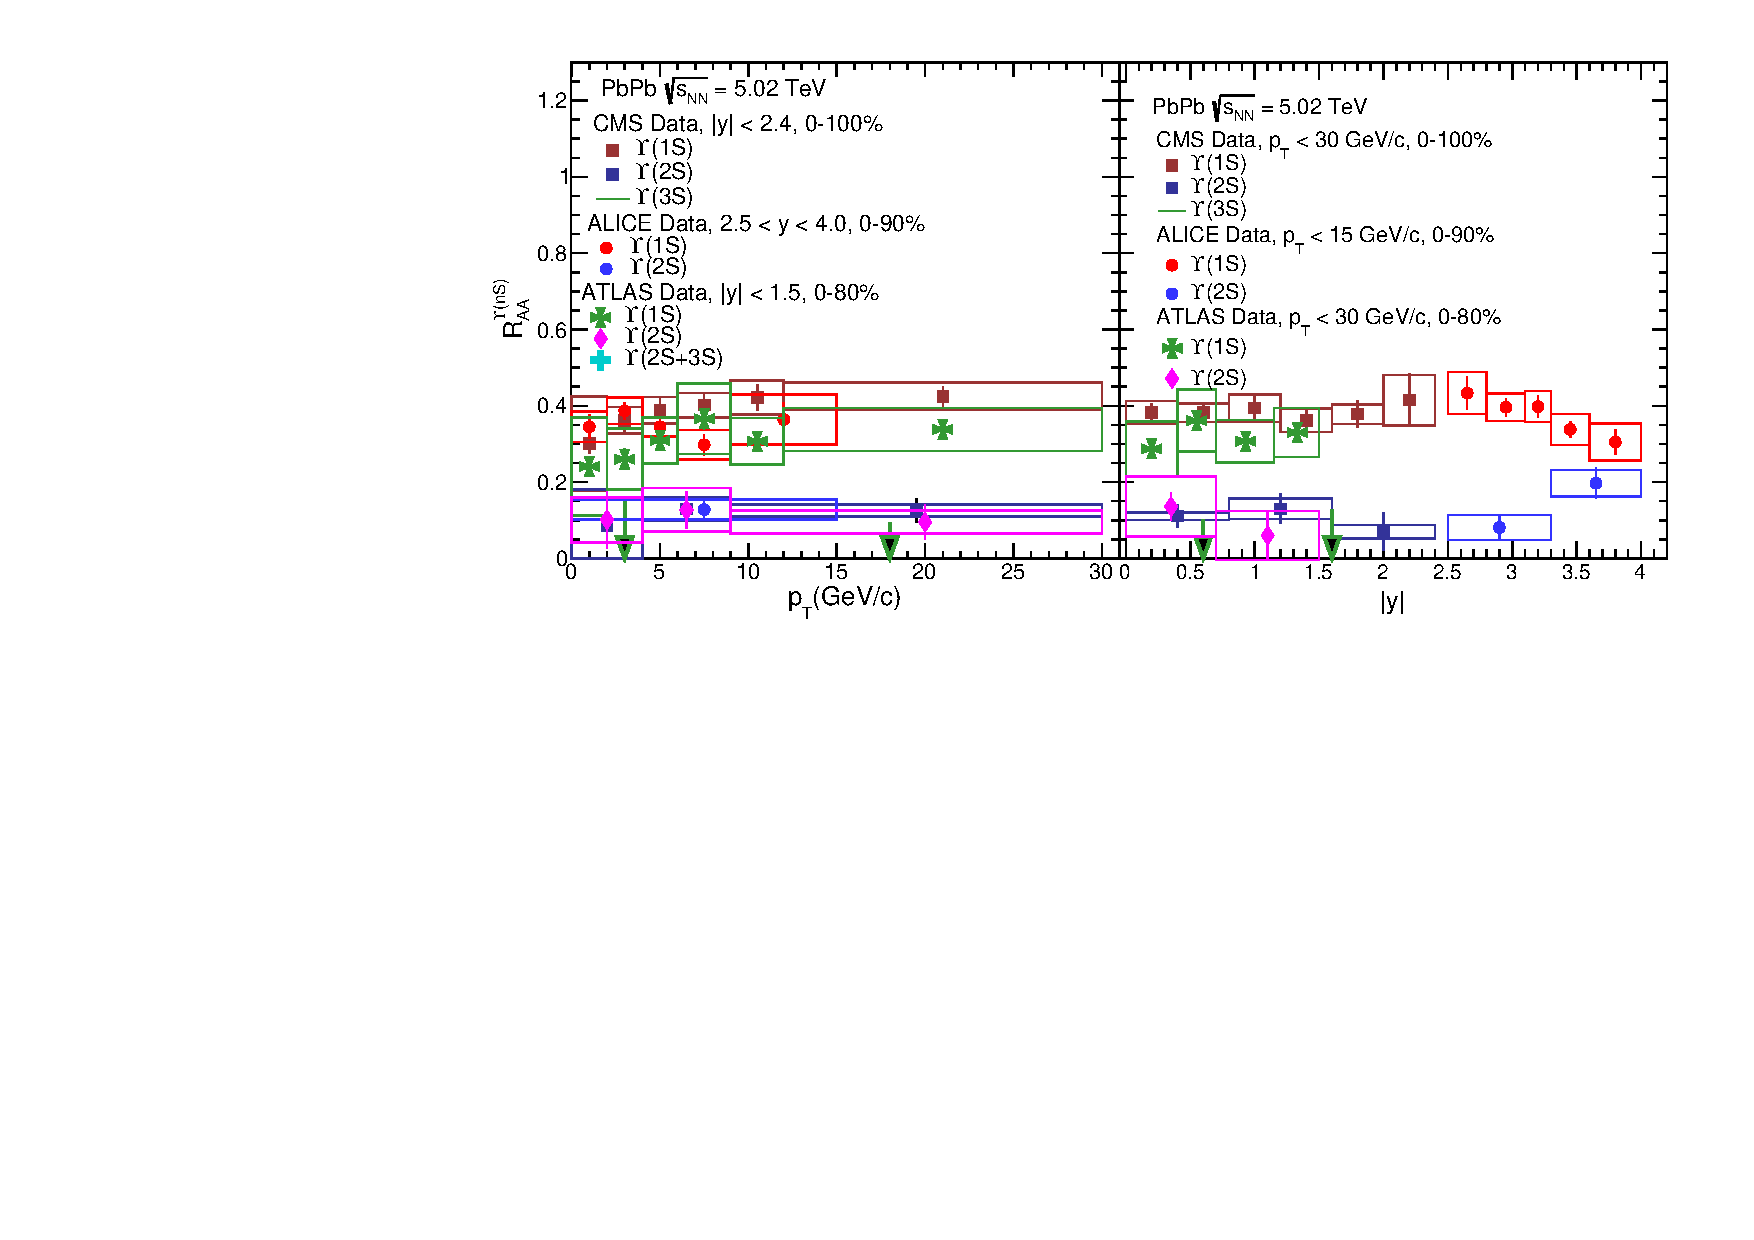
\includegraphics[width=0.99\textwidth]{Figures/ExpOverview/Fig_LHC_YnSRAAPtRap.pdf}
  \caption{(Color online) The $\Upsilon$(nS) nuclear modification factor, $R_{AA}$, (a) as a function of transverse momentum $p_{T}$
    and (b) as a function of rapidity measured by CMS~\cite{CMS:2018zza}, ALICE~\cite{ALICE:2020wwx}
    and ATLAS experiments~\cite{ALICE:2020wwx}.
    The vertical bars denote statistical uncertainties, and the rectangular boxes show the total systematic uncertainties.
  }
  \label{fig:LHCYnSRAAPtRap}
\end{figure}


\begin{figure}
  \begin{center}
  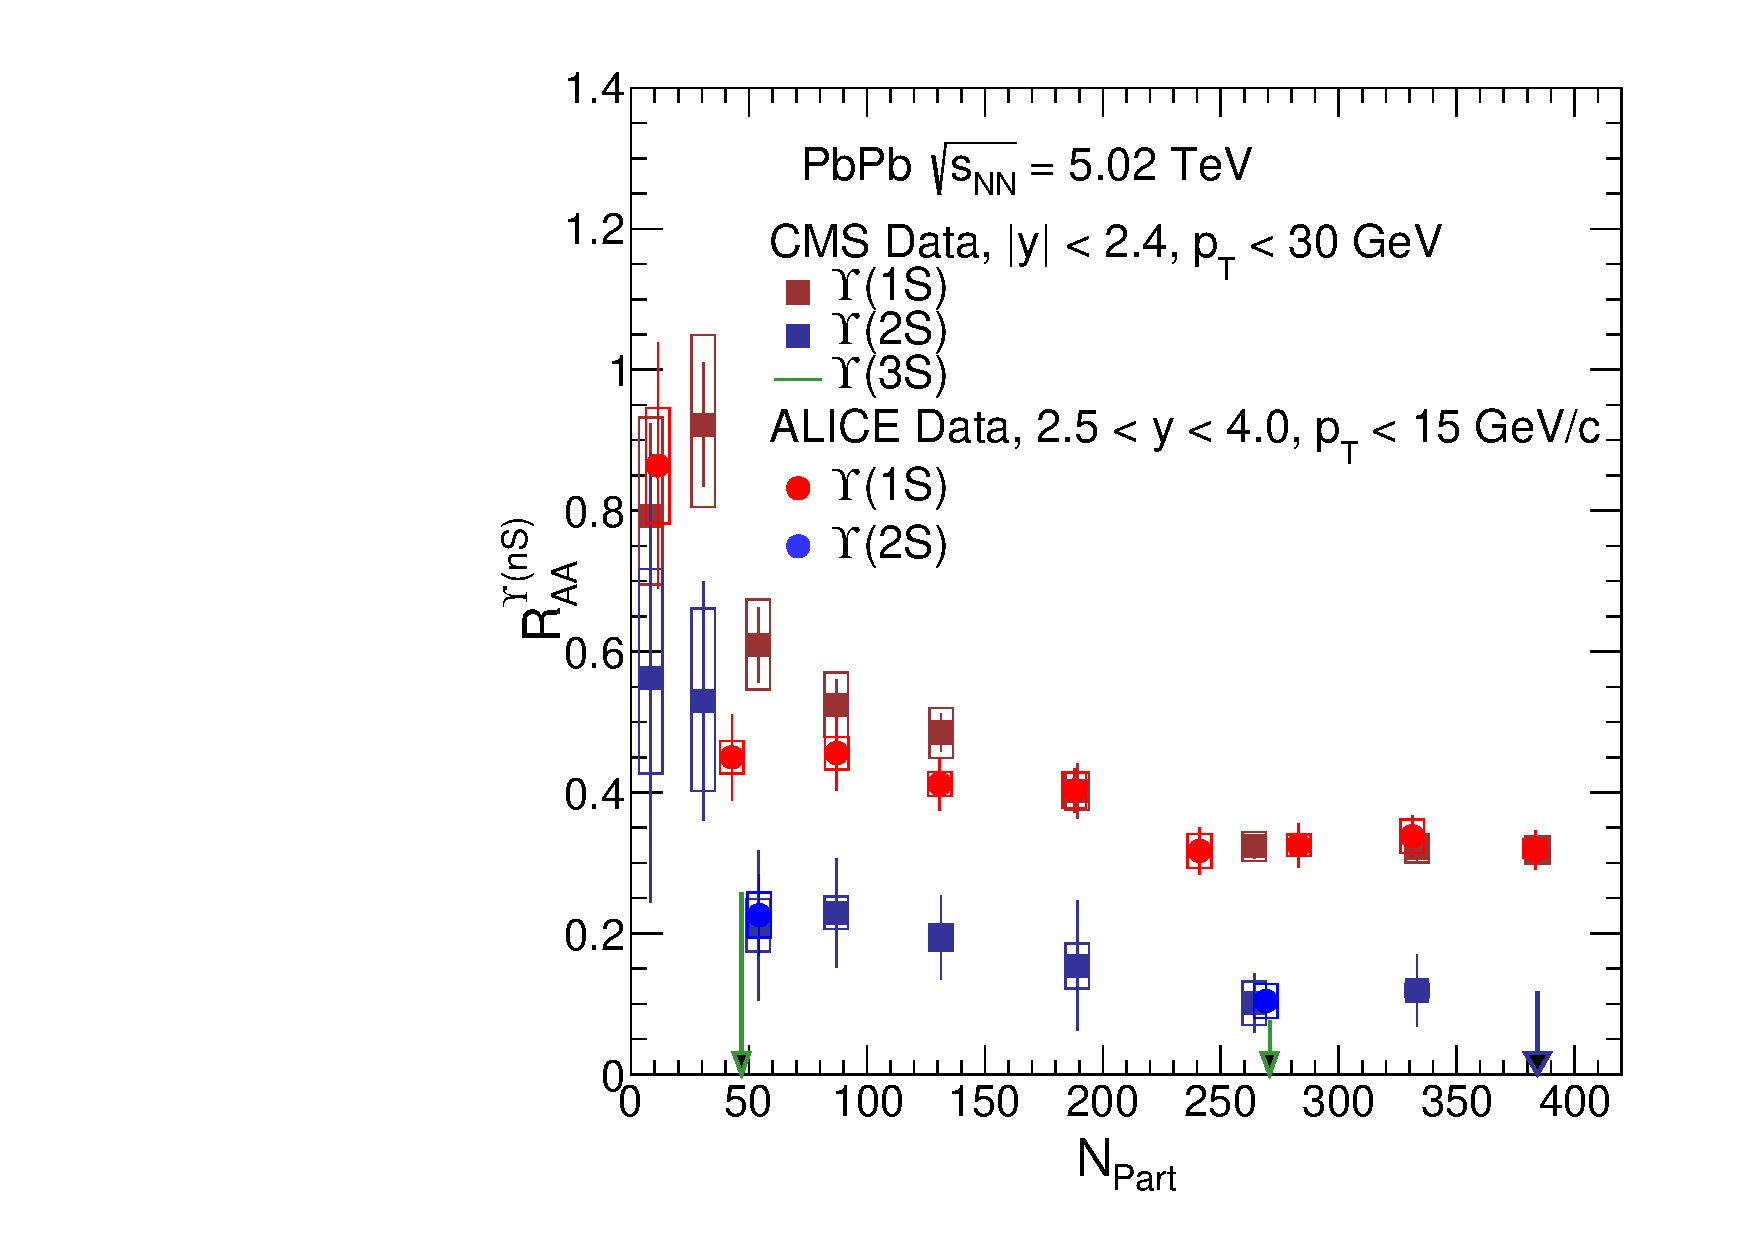
\includegraphics[width=0.6\textwidth]{Figures/ExpOverview/Fig_LHC_YnSRAANPart.pdf}
  %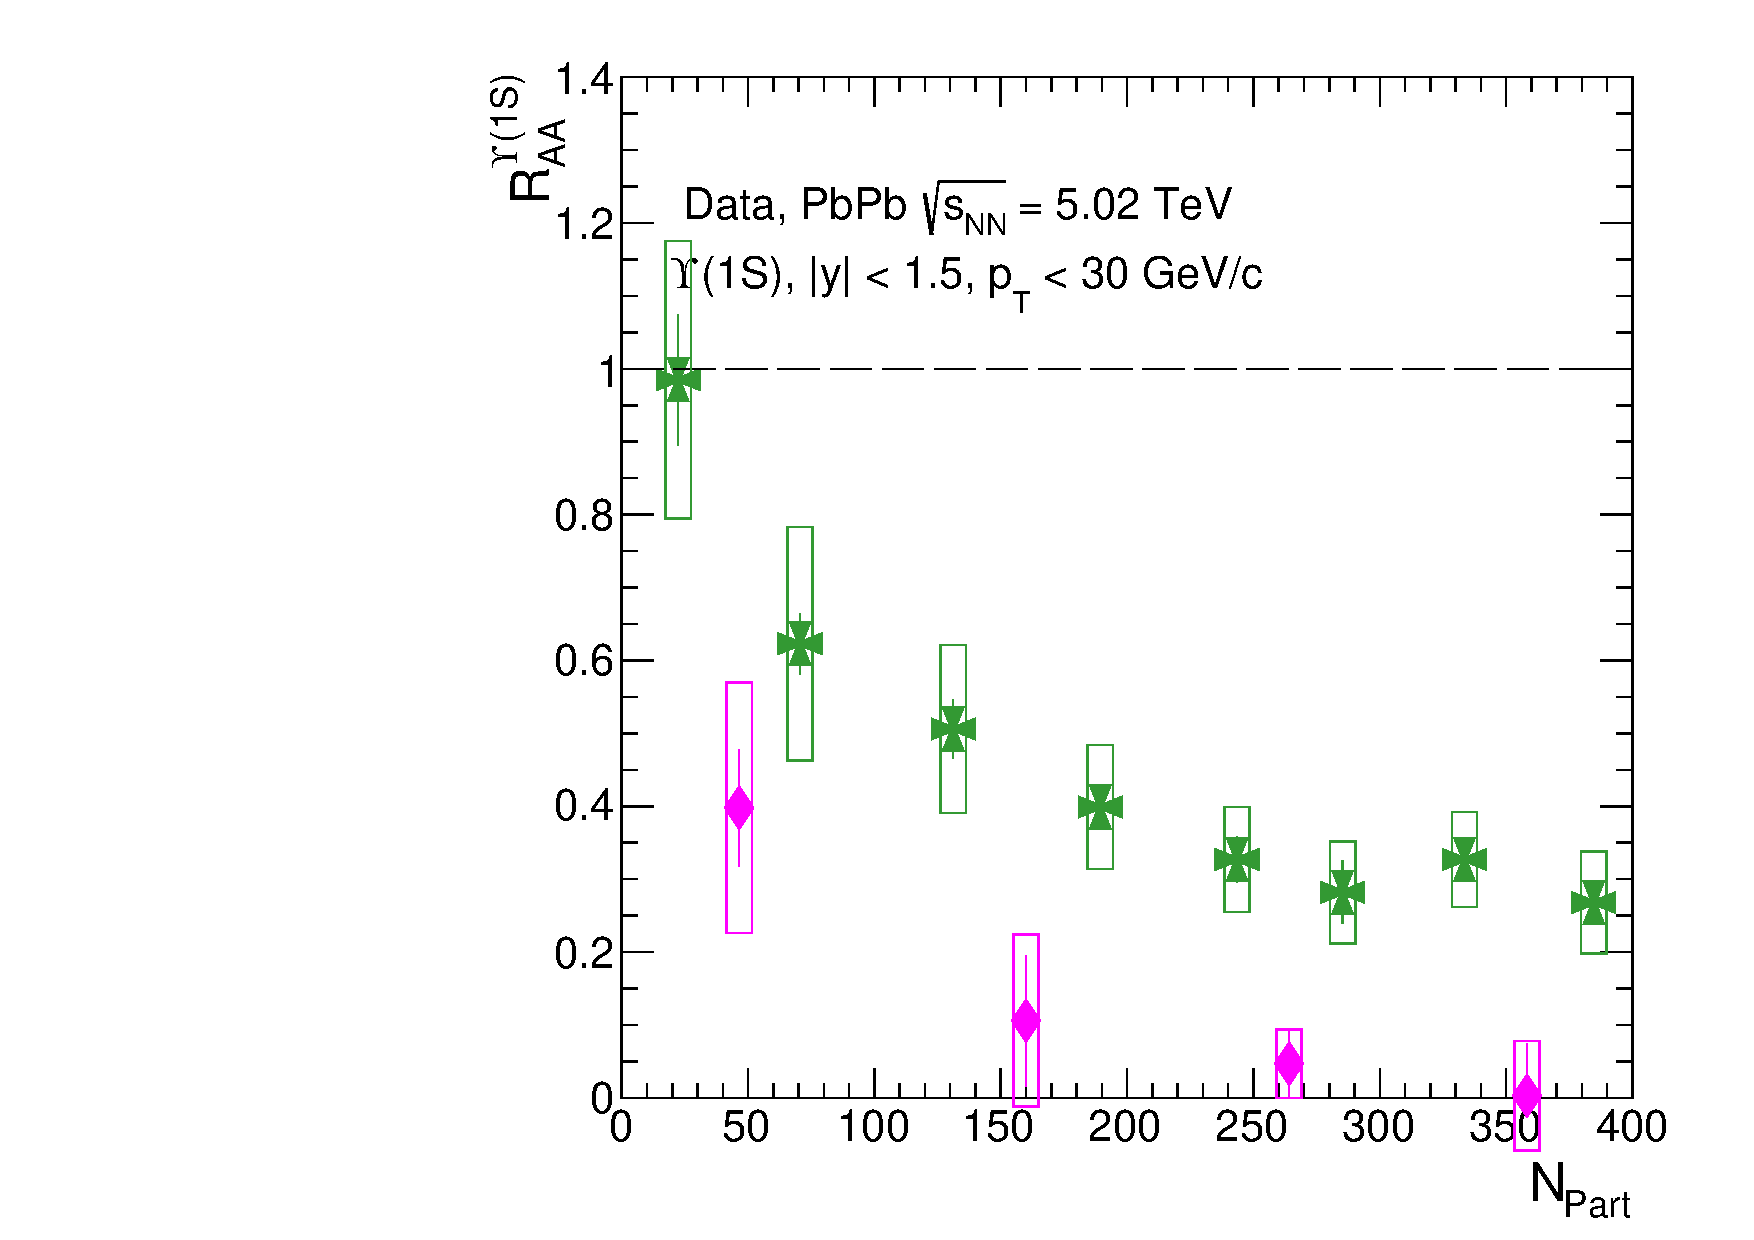
\includegraphics[width=0.49\textwidth]{Figures/ExpOverview/Fig_ATLAS_YnSRAACent_temp.pdf}
  \caption{(Color online) The $\Upsilon$(nS) nuclear modification factor, $R_{AA}$ as a function of N$_{\rm Part}$
    measured by CMS~\cite{CMS:2018zza}, ALICE experiments~\cite{ALICE:2020wwx} and ATLAS experiments~\cite{ALICE:2020wwx}.
    The vertical bars denote statistical uncertainties and the rectangular boxes show the total systematic uncertainties.
  }
  \label{fig:LHCYnSRAANPart}
  \end{center}
\end{figure}



\begin{figure}
  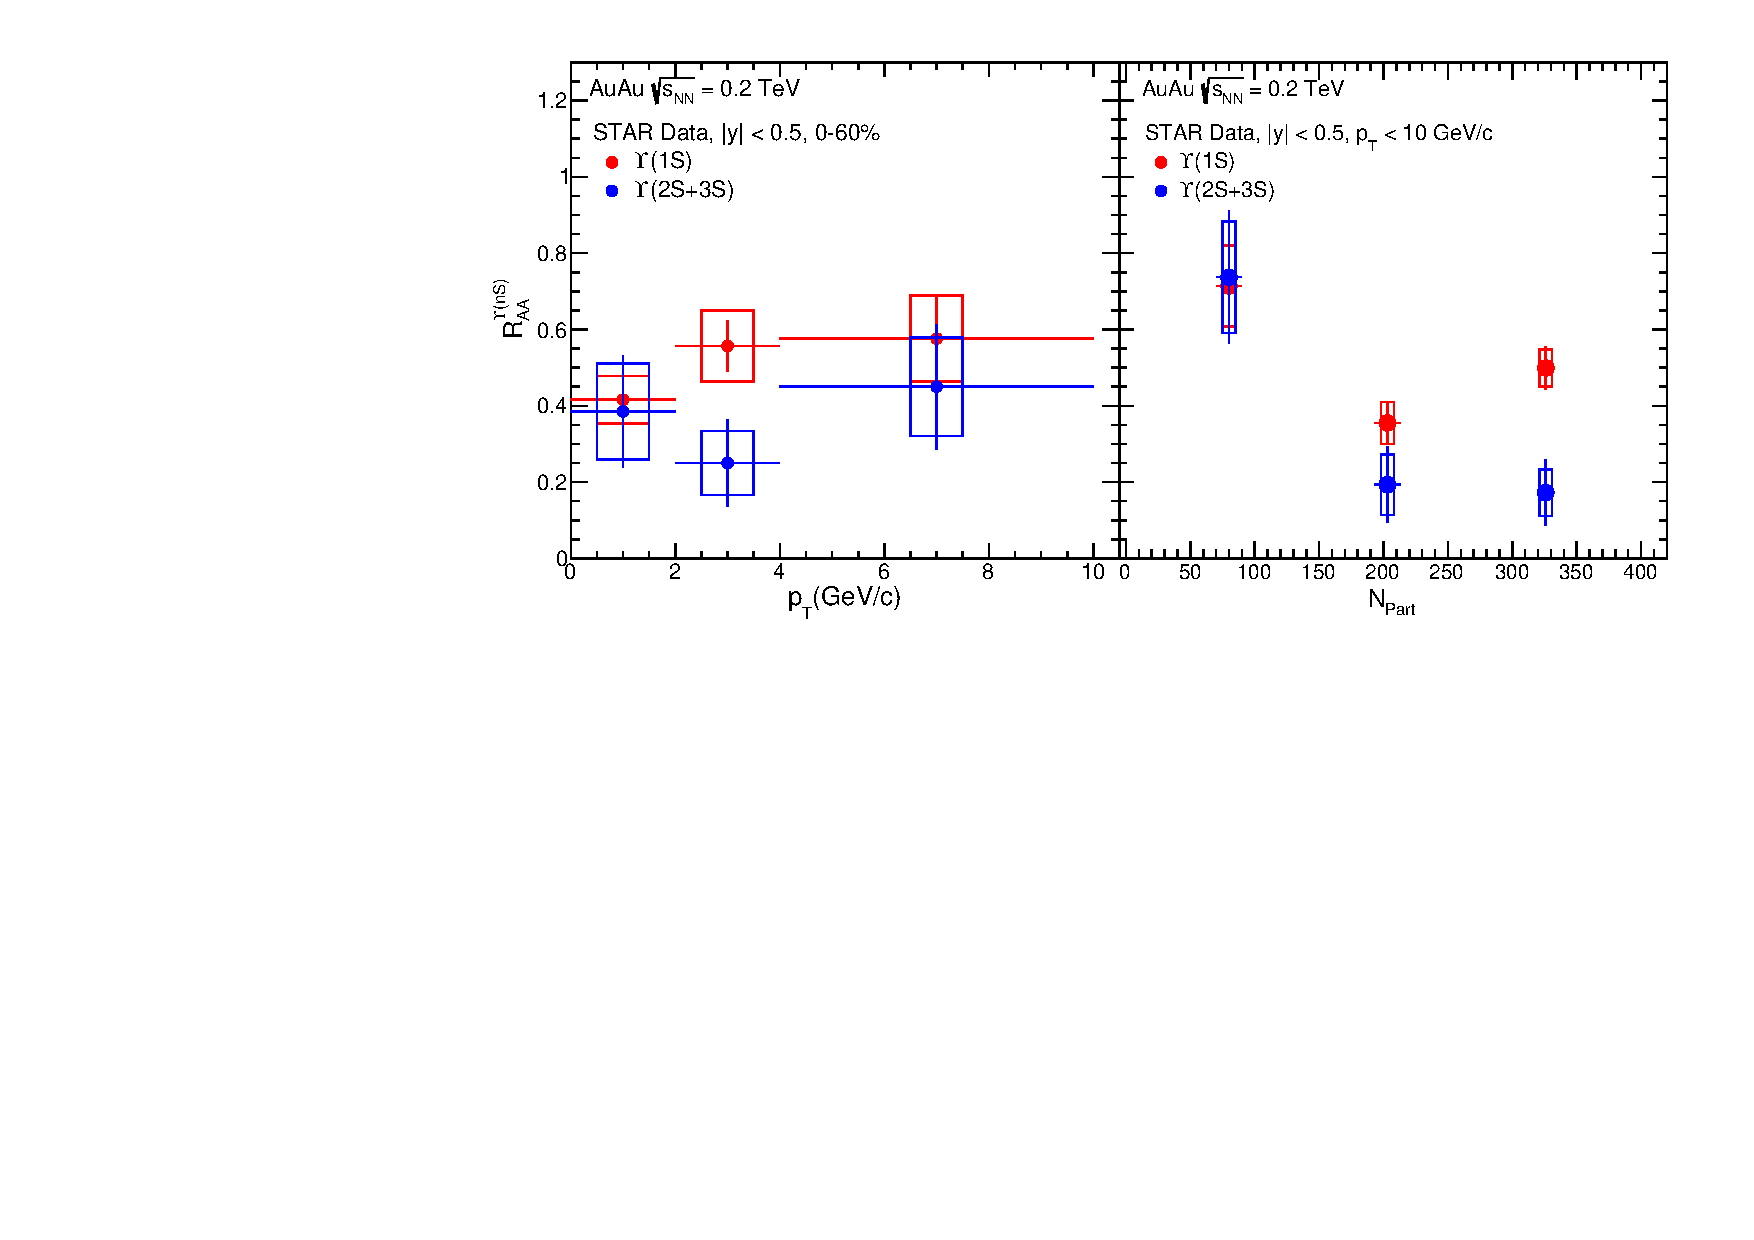
\includegraphics[width=0.99\textwidth]{Figures/ExpOverview/Fig_RHIC_YnSRAAPt.pdf}
  \caption{(Color online) The $\Upsilon$(nS) nuclear modification factor, $R_{AA}$, (a) as a function of transverse momentum $p_{T}$
    and (b) as a function of N$_{\rm Part}$ measured by STAR experiments~\cite{Wang:2019vau}. The vertical bars denote
    statistical uncertainties, and the rectangular boxes show the total systematic uncertainties.
  }
  \label{fig:RHICYnSRAAPt}
\end{figure}



\begin{figure}
  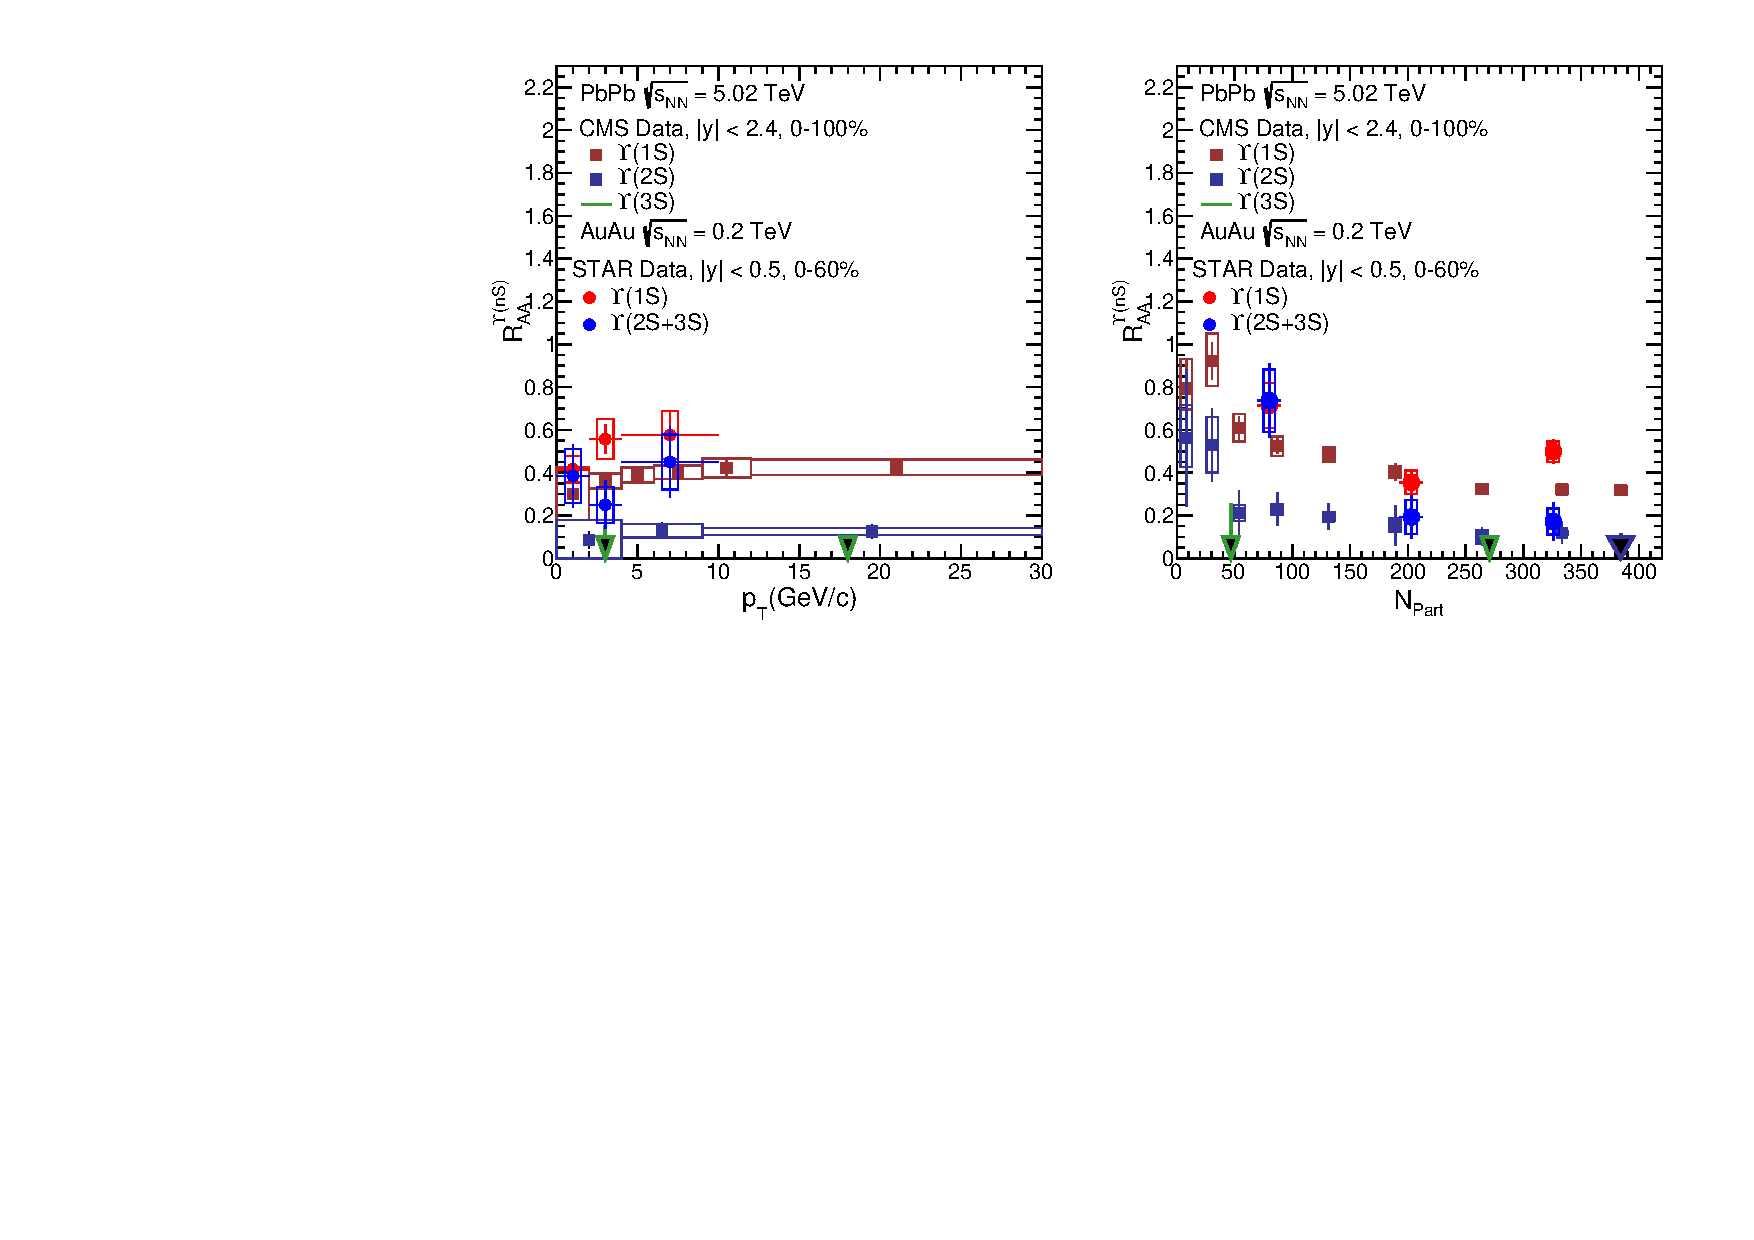
\includegraphics[width=0.99\textwidth]{Figures/ExpOverview/Fig_RHIC_LHC_YnSRAA.pdf}
  \caption{(Color online) The $\Upsilon$(nS) nuclear modification factor, $R_{AA}$, (a) as a function of transverse momentum $p_{T}$
    and (b) as a function of N$_{\rm Part}$ measured by STAR experiments~\cite{Wang:2019vau} at 0.2 TeV and CMS experiment~\cite{CMS:2018zza} at 5.5 TeV.
    The vertical bars denote statistical uncertainties, and the rectangular boxes show the total systematic uncertainties.
  }
  \label{fig:RHICYnSRAANPart}
\end{figure}


Figure~\ref{fig:LHCYnSRAAPtRap} shows
    the $\Upsilon$(nS) nuclear modification factor, $R_{AA}$, (a) as a function of transverse momentum $p_{T}$
    and (b) as a function of rapidity measured by CMS~\cite{CMS:2018zza}, ALICE~\cite{ALICE:2020wwx}
    and ATLAS experiments~\cite{ALICE:2020wwx}.
    The vertical bars denote statistical uncertainties, and the rectangular boxes show the total systematic uncertainties.

Figure~\ref{fig:LHCYnSRAANPart} shows
  the $\Upsilon$(nS) nuclear modification factor, $R_{AA}$ as a function of N$_{\rm Part}$
    measured by CMS~\cite{CMS:2018zza}, ALICE experiments~\cite{ALICE:2020wwx} and ATLAS experiments~\cite{ALICE:2020wwx}.
    The vertical bars denote statistical uncertainties and the rectangular boxes show the total systematic uncertainties.

Figure~\ref{fig:RHICYnSRAAPt} shows
  the $\Upsilon$(nS) nuclear modification factor, $R_{AA}$, (a) as a function of transverse momentum $p_{T}$
    and (b) as a function of N$_{\rm Part}$ measured by STAR experiments~\cite{Wang:2019vau}. The vertical bars denote
    statistical uncertainties, and the rectangular boxes show the total systematic uncertainties.


Figure~\ref{fig:RHICYnSRAANPart} shows
  the $\Upsilon$(nS) nuclear modification factor, $R_{AA}$, (a) as a function of transverse momentum $p_{T}$
  and (b) as a function of N$_{\rm Part}$ measured by STAR experiments~\cite{Wang:2019vau} at 0.2 TeV and
  CMS experiment~\cite{CMS:2018zza} at 5.5 TeV. The vertical bars denote statistical uncertainties, and the
  rectangular boxes show the total systematic uncertainties.


\begin{figure}
  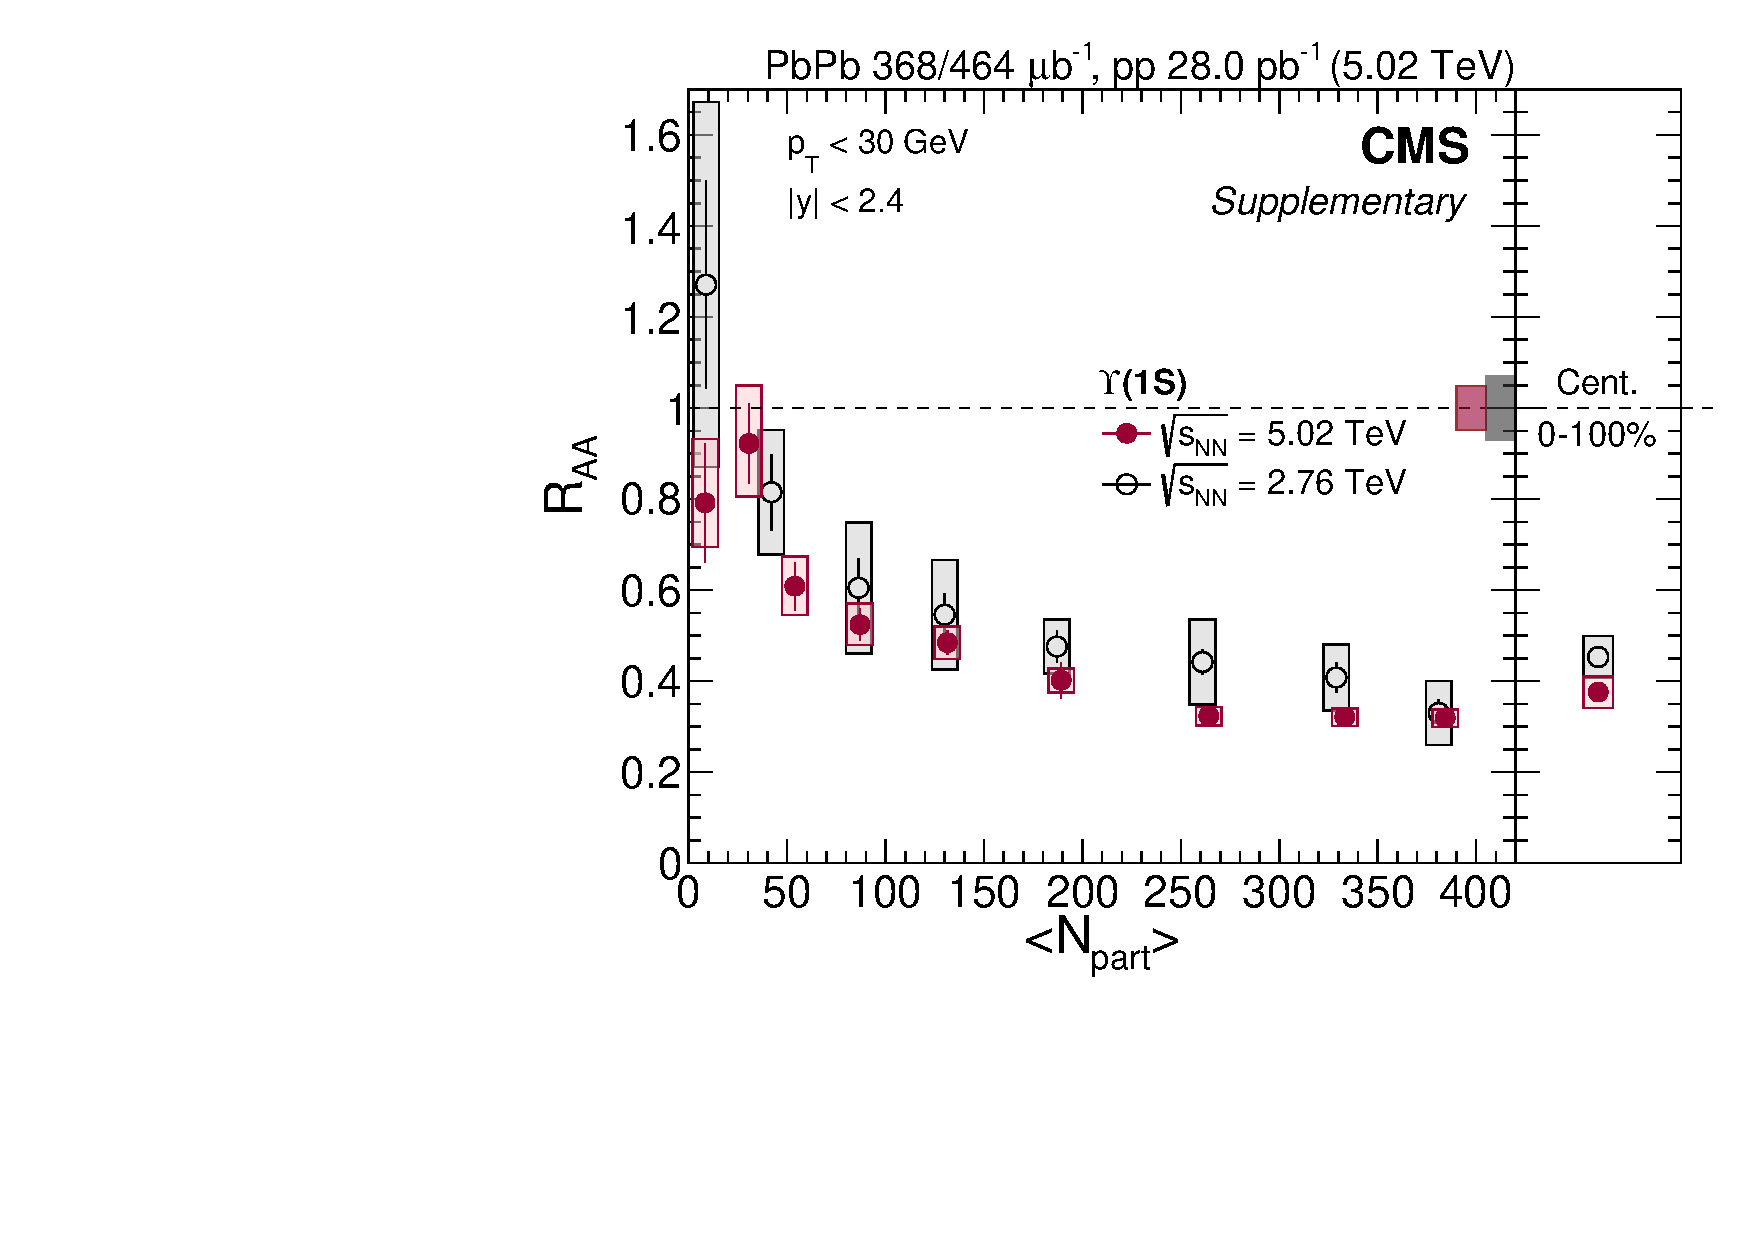
\includegraphics[width=0.49\textwidth]{Figures/ExpOverview/CMS-HIN-16-023_Figure-aux_001.pdf}
    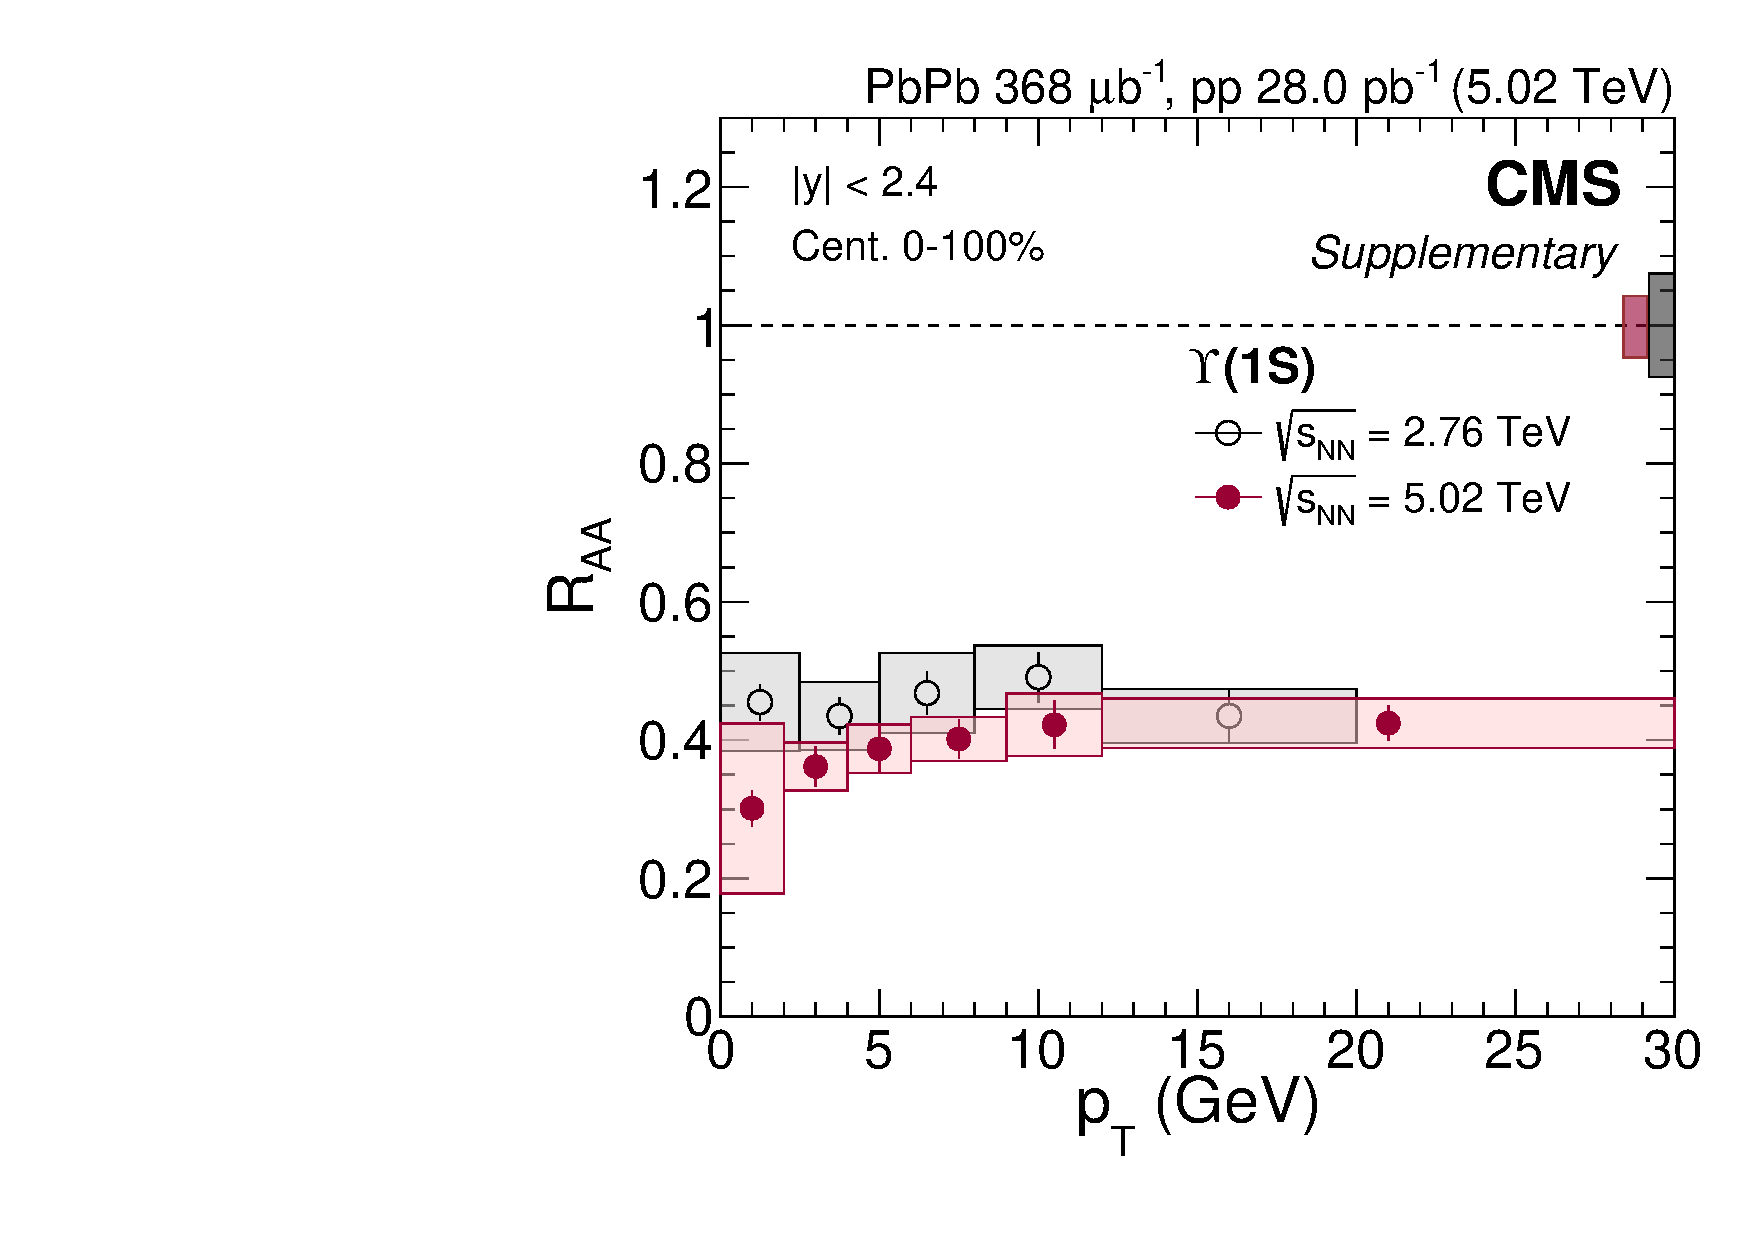
\includegraphics[width=0.49\textwidth]{Figures/ExpOverview/CMS-HIN-16-023_Figure-aux_002.pdf}
  \caption{(Color online) The $\Upsilon$(nS) nuclear modification factor, $R_{AA}$, (a) as a function of transverse momentum $p_{T}$
    and (b) as a function N$_{\rm Part}$ measured by CMS
    at 2.76~\cite{Khachatryan:2016xxp} and 5.02 TeV~\cite{CMS:2018zza}
  }
  \label{fig:LHCYnSRAAenergy}
\end{figure}

Figure~\ref{fig:LHCYnSRAAenergy} shows 
  the $\Upsilon$(nS) nuclear modification factor, $R_{AA}$, (a) as a function of transverse momentum $p_{T}$
  and (b) as a function N$_{\rm Part}$ measured by CMS
    at 2.76~\cite{Khachatryan:2016xxp} and 5.02 TeV~\cite{CMS:2018zza}
  

  
    
\subsection{$\Upsilon$(nS) azimuthal anisotropy}

The screening due to the QGP can also result in an azimuthal asymmetry in the observed yields of quarkonia. In non-central
heavy ion collisions, the produced QGP has a lenticular shape in the transverse plane. Consequently, the average path length
for quarkonia traveling through the medium depends on the direction taken with respect to this shape, with a larger suppression
in the direction of the longer axis~\cite{He:2015hfa}. The anisotropic distribution of particles can be characterized by the magnitudes
of the Fourier co-efficients (v$_{n}$) of the azimuthal correlation of particles~\cite{Voloshin:1994mz}. By studying the
azimuthal distribution of the quarkonia, it is possible to develop a more comprehensive understanding of the dynamics of their
production.

\begin{figure}
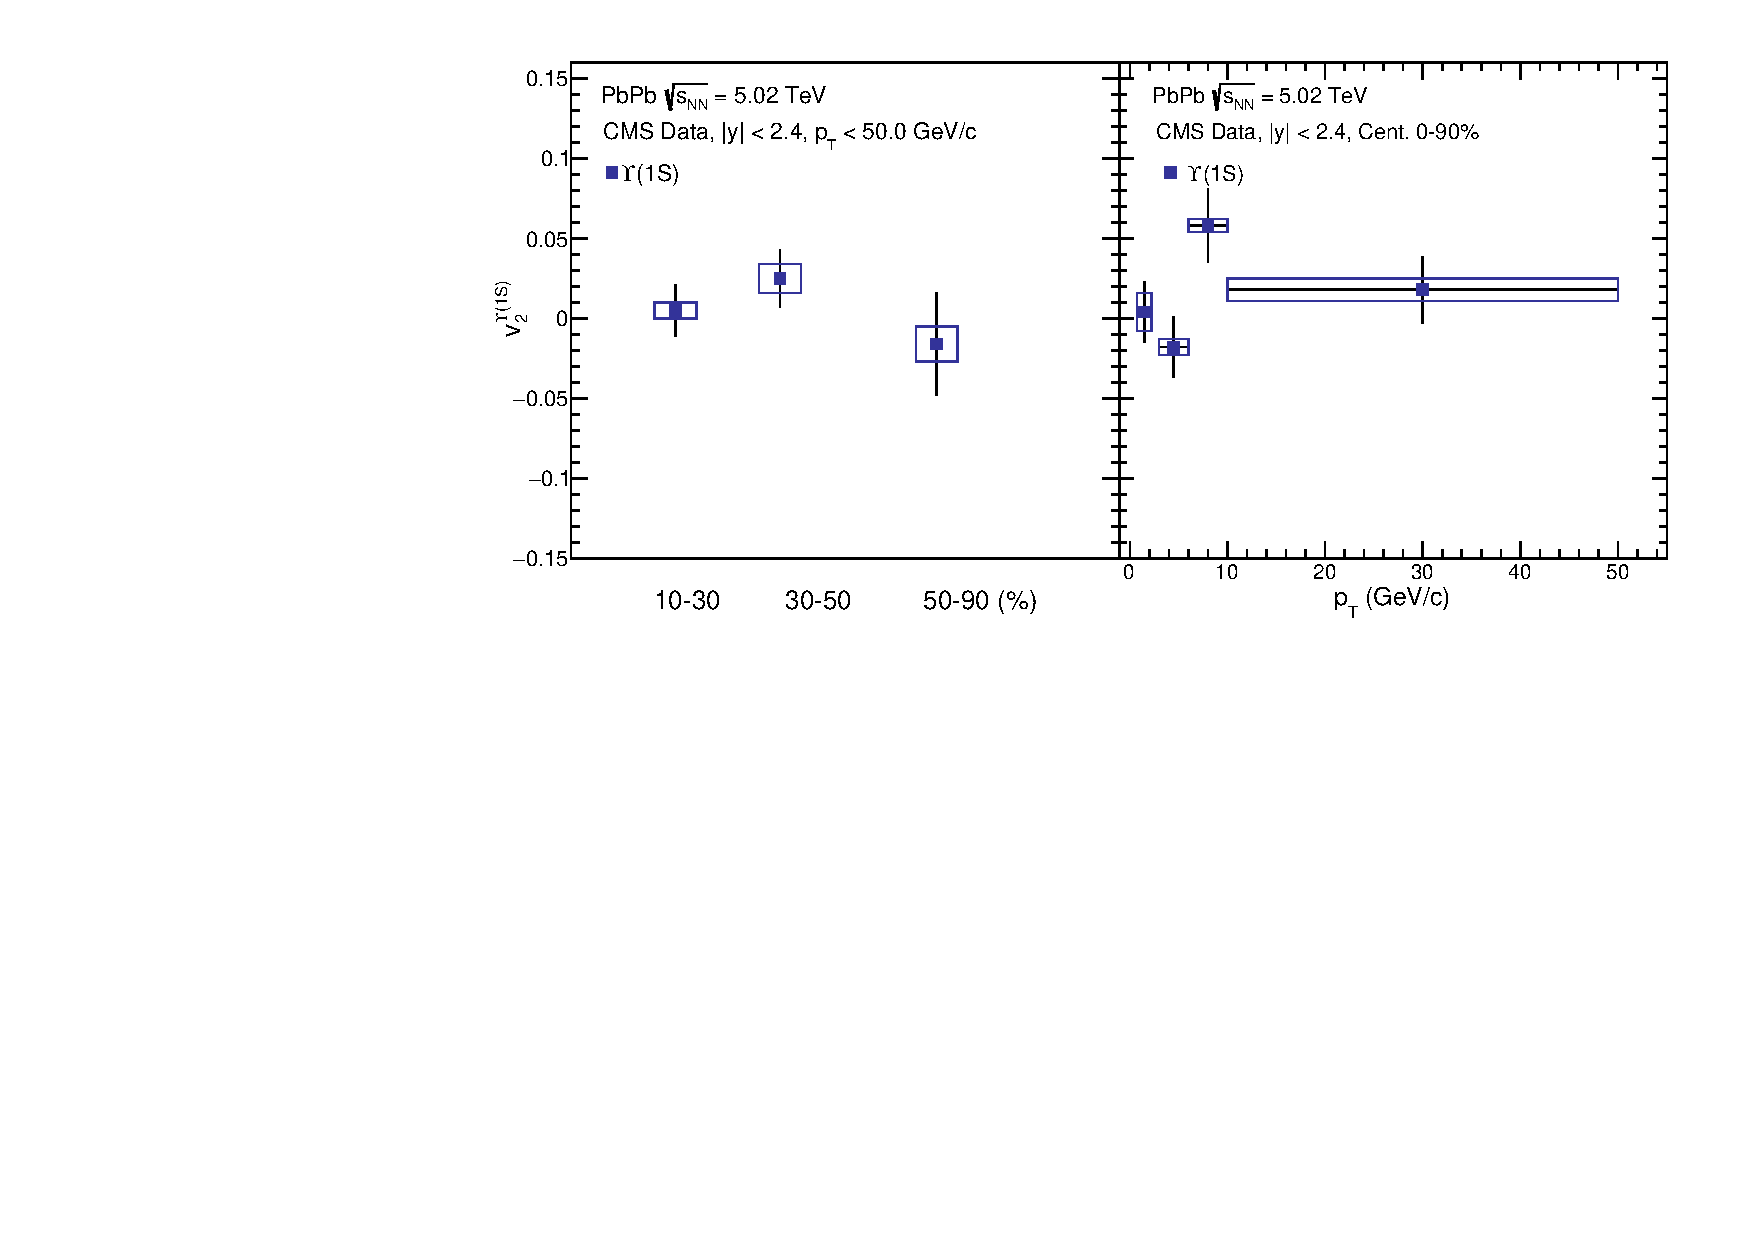
\includegraphics[width=0.99\textwidth]{Figures/ExpOverview/Fig_CMS_Y1S_5TeV_V2.pdf}
\caption{(Color online) The $\Upsilon$(1S) azimuthal anisotropy (v$_{2}$) (a) as a function of collision centrality and 
  (b) as a function of transverse momentum $p_{T}$~\cite{CMS:2020efs}. The vertical bars denote statistical uncertainties,
  and the rectangular boxes show the total systematic uncertainties.
}
\label{fig:Upsilon1SV2CMS}
\end{figure}



The CMS experiment measured v$_{2}$ coefficients for $\Upsilon$(1S) and $\Upsilon$(2S) mesons in PbPb collisions
at a nucleon-nucleon center-of-mass energy of 5.02TeV. Figure~\ref{fig:Upsilon1SV2CMS} shows the $\Upsilon$(1S) azimuthal
anisotropy (v$_{2}$) (a) as a function of collision centrality and (b) as a function of transverse momentum $p_{T}$ measured
by CMS experiment at LHC~\cite{CMS:2020efs}. The p$_{T}$ integrated results
shown in Fig.~\ref{fig:Upsilon1SV2CMS} (a) for three centrality intervals are consistent with zero within the statistical
uncertainties. The average v$_{2}$ values in the 10-90$\%$ centrality interval measured by CMS experiment are found to
be 0.007$\pm$0.011(stat)$\pm$0.005(syst) for $\Upsilon$(1S) and -0.063$\pm$0.085(stat)$\pm$0.037(syst) for $\Upsilon$(2S).   
The p$_{T}$ dependence of $\Upsilon$(1S) meson v$_{2}$ values is measured for the 10-90$\%$ centrality interval.
The v$_{2}$ values are consistent with zero in the measured p$_T$ range, except for the 6$<$p$_{T}<$10 GeV/c interval that
shows a 2.6$\sigma$ deviation from zero. 

\begin{figure}
  \begin{center}
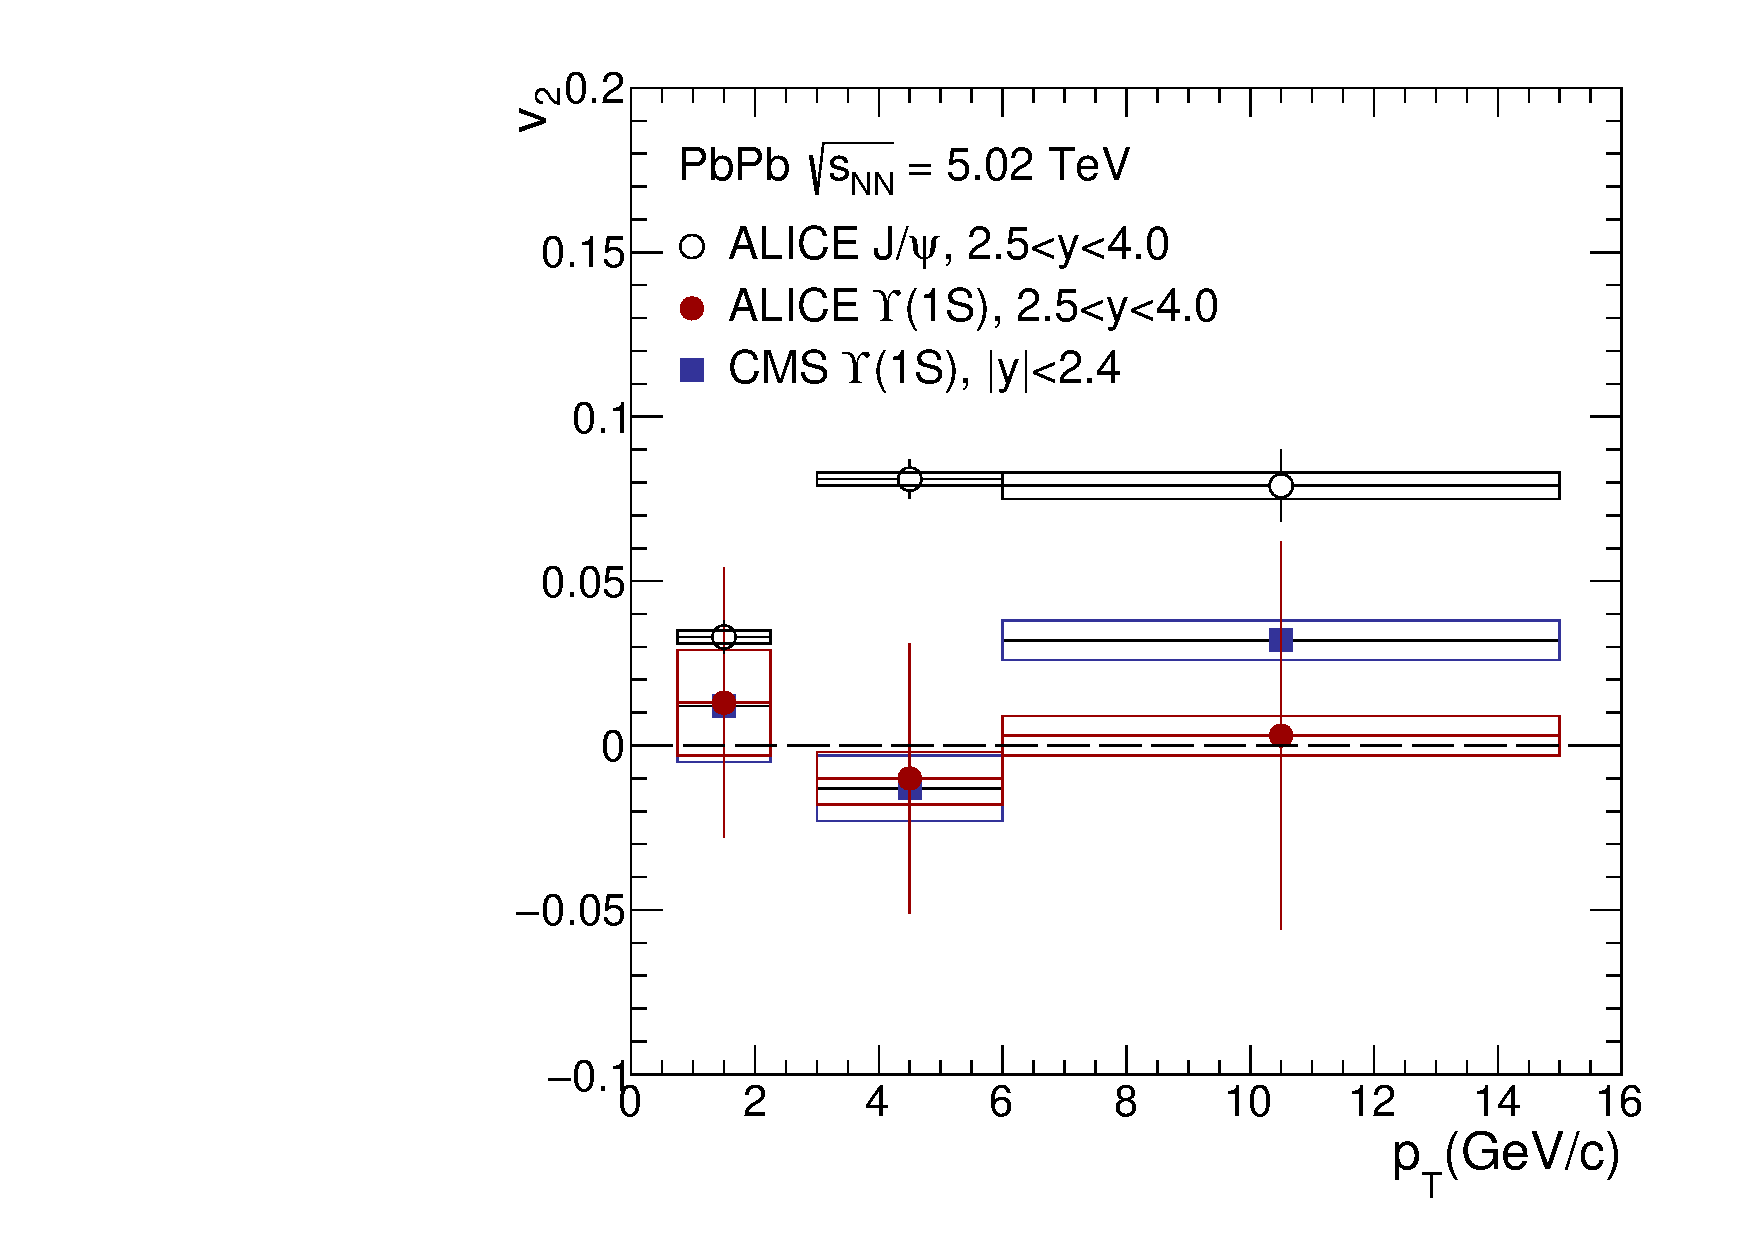
\includegraphics[width=0.6\textwidth]{Figures/ExpOverview/Fig_CMS_ALICE_Y1S_5TeV_V2.pdf}
\caption{(Color online) The v$_{2}$ for $\Upsilon$(1S) mesons as a function of p$_{T}$ in the
  rapidity range $|y|<2.4$ measured by
  CMS experiment~\cite{CMS:2020efs} compared with the ALICE results for $Upsilon$(1S) and J/$\psi$ mesons measured
  in 2.5$<$y$<$4~\cite{ALICE:2019pox}. The vertical bars denote statistical uncertainties,
  and the rectangular boxes show the total systematic uncertainties.
}
\label{fig:Upsilon1SV2Compare}
\end{center}
\end{figure}

Figure~\ref{fig:Upsilon1SV2Compare} shows the p$_{T}$ differential results for v$_{2}$ of $\Upsilon$(1S)
mesons measured by CMS experiment along with the measurements of v$_{2}$ for $\Upsilon$(1S) and J/$\psi$
from ALICE in the same p$_{T}$ (0-15 GeV/c) and centrality (5-60$\%$) interval. The measurements from CMS
and ALICE are done in complementary rapidity ranges. The $\Upsilon$(1S) V$_{2}$ is consistant with zero while
the J/$\psi$ meson measured by ALICE in same kinematic conditions have finite v$_{2}$. Together, the CMS and ALICE
results indicate that the geometry of the medium has little influence on the $\Upsilon$(1S) yields and recombination is
not a dominant process in the production of this meson. The results also indicate that the path-length dependence of
$\Upsilon$(1S) suppression is small.



\subsection{$\Upsilon$(nS) R$_{pA}$ }

CMS measured the $Upsilon$ ratios as a function of event activity measured in 
in $\sqrt{s_{NN}}$=5.02 TeV pPb~\cite{CMS:2013jsu} and compared with $\sqrt{s}$=2.76 TeV pp
and PPb Collisions.
 The nuclear modification of all $\Upsilon$ states is also measured in pPb collisions
 at $\sqrt{s_\mathrm{NN}}$ = 5.02 TeV~\cite{CMS:2022wfi}.
 Recently, relative production of $\Upsilon$(nS) states are measured as a function of
 event activity in proton-proton collisions at $ \sqrt{s} $ = 7 TeV~\cite{CMS:2020fae}

   


\begin{figure}
  \begin{center}
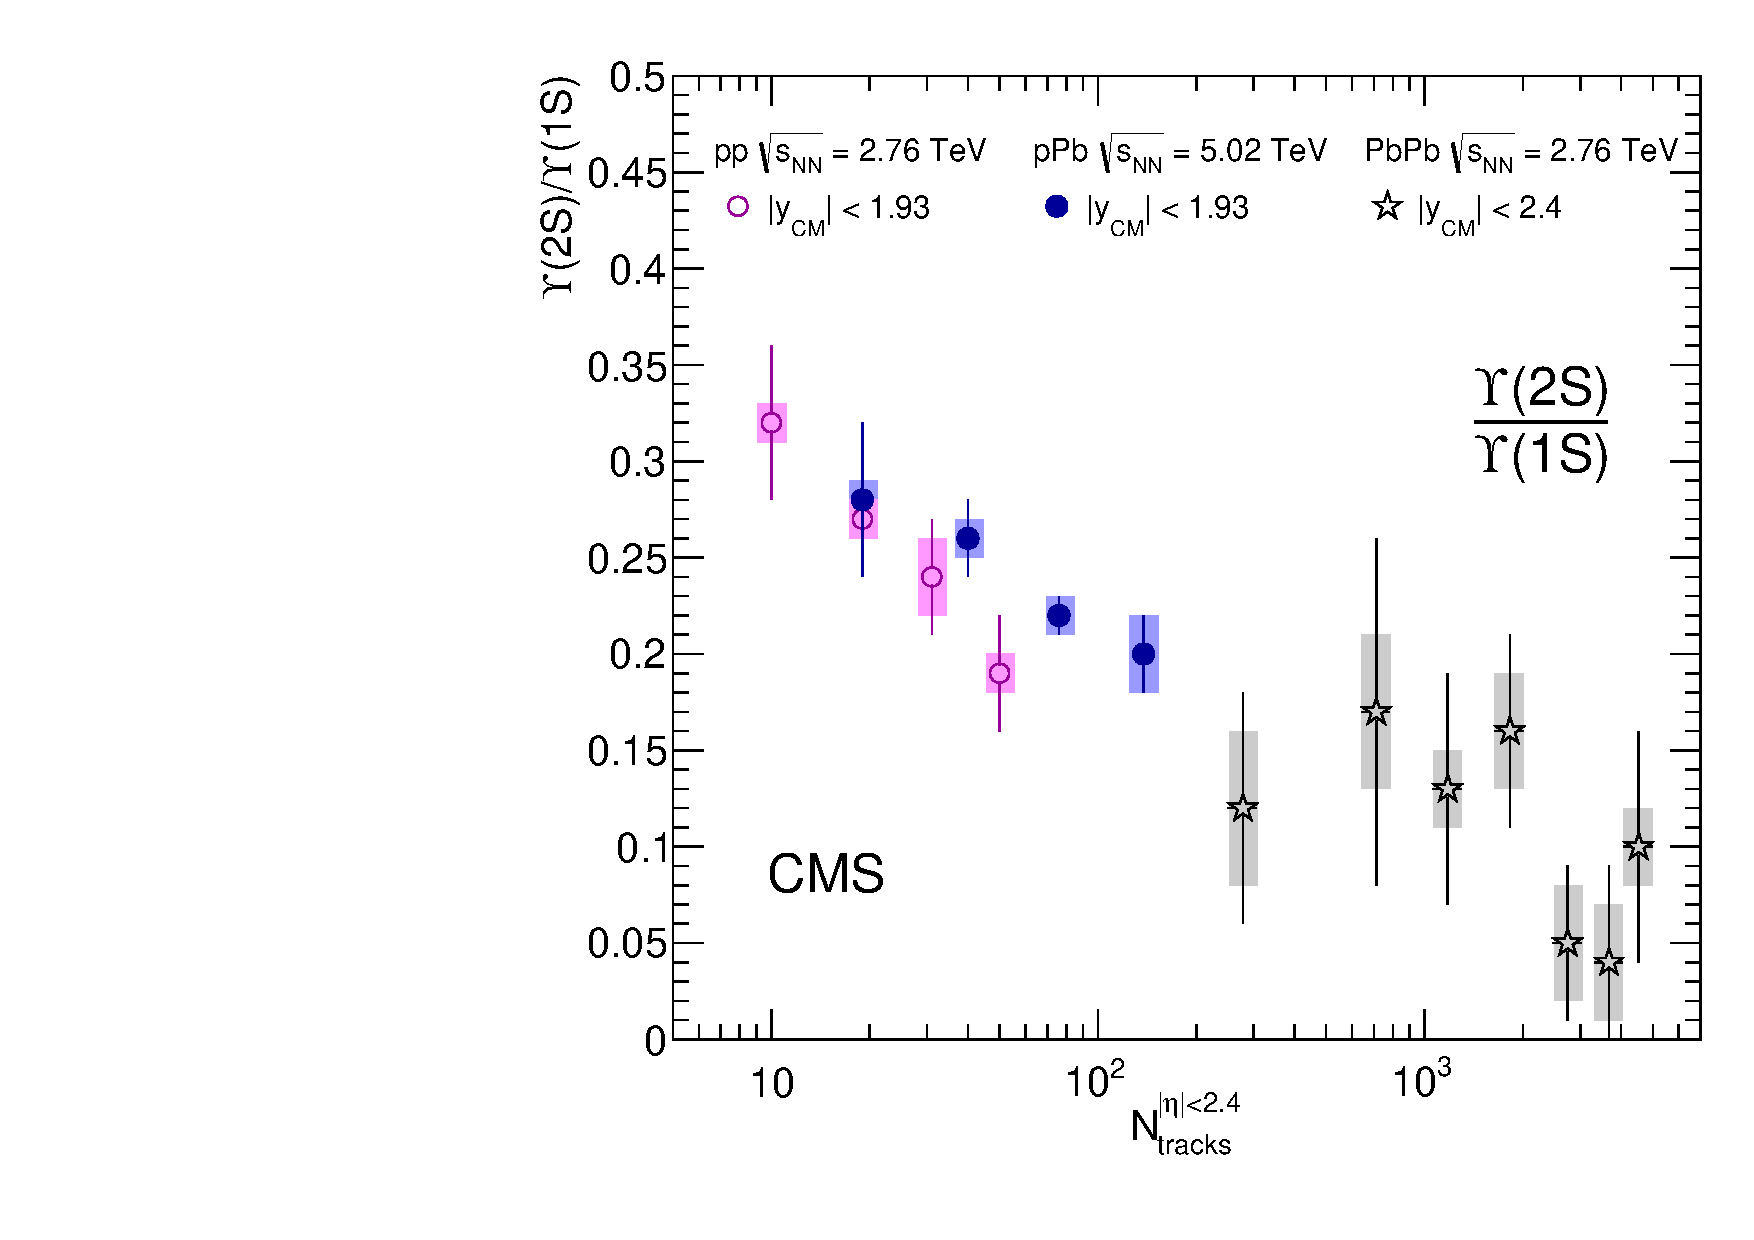
\includegraphics[width=0.49\textwidth]{Figures/ExpOverview/Fig_trk_pPb.pdf}
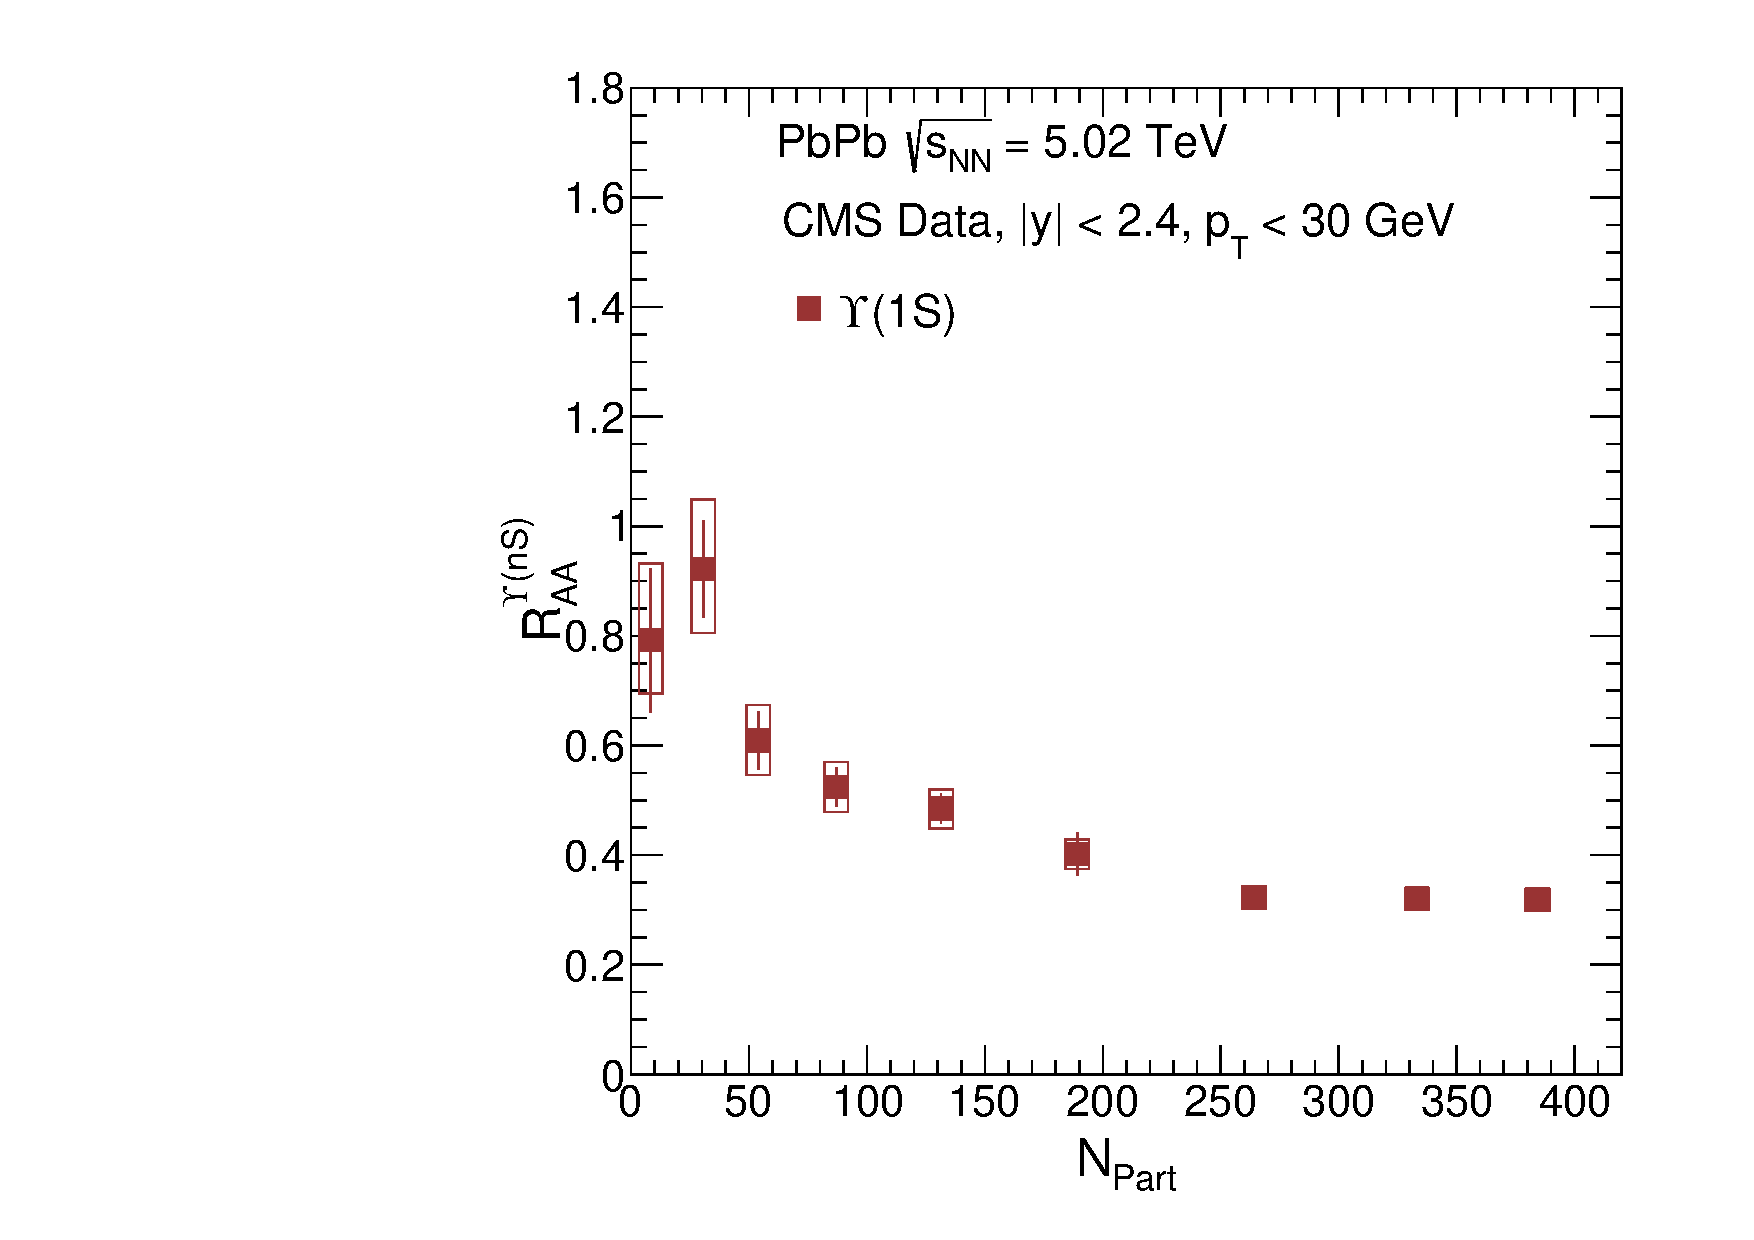
\includegraphics[width=0.49\textwidth]{Figures/ExpOverview/Fig_CMS_Y1SRAANPart.pdf}
\caption{(Color online)
  (a) The ratio $\Upsilon$(2S)/$\Upsilon$(1S) as a function of event activity measured in 
$\sqrt{s_{NN}}$=5.02 TeV pPb collisions~\cite{CMS:2013jsu} and is compared with pp
and PbPb Collisions at $\sqrt{s_{NN}}$=2.76 TeV.
(b) The $\Upsilon$(nS) nuclear modification factor, $R_{AA}$ as a function of $N_{\rm Part}$
at $\sqrt{s_{NN}}$=5.02 TeV measured by CMS~\cite{CMS:2018zza}.
}
\label{fig:UpsilonpPb}
\end{center}
\end{figure}

Figure~\ref{fig:UpsilonpPb}(a) shows
the ratio $\Upsilon$(2S)/$\Upsilon$(1S) as a function of event activity measured in 
$\sqrt{s_{NN}}$=5.02 TeV pPb collisions~\cite{CMS:2013jsu} and is compared with pp
and PbPb Collisions at $\sqrt{s_{NN}}$=2.76 TeV.
Figure~\ref{fig:UpsilonpPb}(b) shows the $\Upsilon$(nS) nuclear modification factor, $R_{AA}$ as a function of $N_{\rm Part}$
at $\sqrt{s_{NN}}$=5.02 TeV measured by CMS~\cite{CMS:2018zza}.

  

The $N_{\rm tracks}$ corresponding to $N_{\rm Part}$ in Fig~\ref{fig:UpsilonpPb} at 5.02 TeV
can be obtained using the $N_{\rm tracks}$ for same $N_{\rm Part}$ given
for 2.76 TeV~\cite{Khachatryan:2016xxp} and scale as 

\begin{equation}
N_{\rm tracks}|_{5.02} =  N_{\rm tracks}|_{2.76} \times \frac{dN/d\eta |_{5.02}} {dN/d\eta|_{2.76}}.
\end{equation}
where $\frac{dN/d\eta |_{5.02}} {dN/d\eta|_{2.76}}$.

The ratio $\Upsilon$(2S)/$\Upsilon$(1S) at $\sqrt{s_{NN}}$=5.02 can be obtained as 

\begin{equation}
\frac{\Upsilon(2S)}{\Upsilon(1S)} = \frac{R_{AA}^{2S}}{R_{AA}^{1S}} \times \frac{\sigma_{pp}^{1S}}{\sigma_{pp}^{2S}}.
\end{equation}

Here $\sigma_{pp}^{1S}$ and $\sigma_{pp}^{2S}$ can be obtained by integrating the pp cross section
measured by CMS~\cite{CMS:2018zza}.


\begin{figure}
  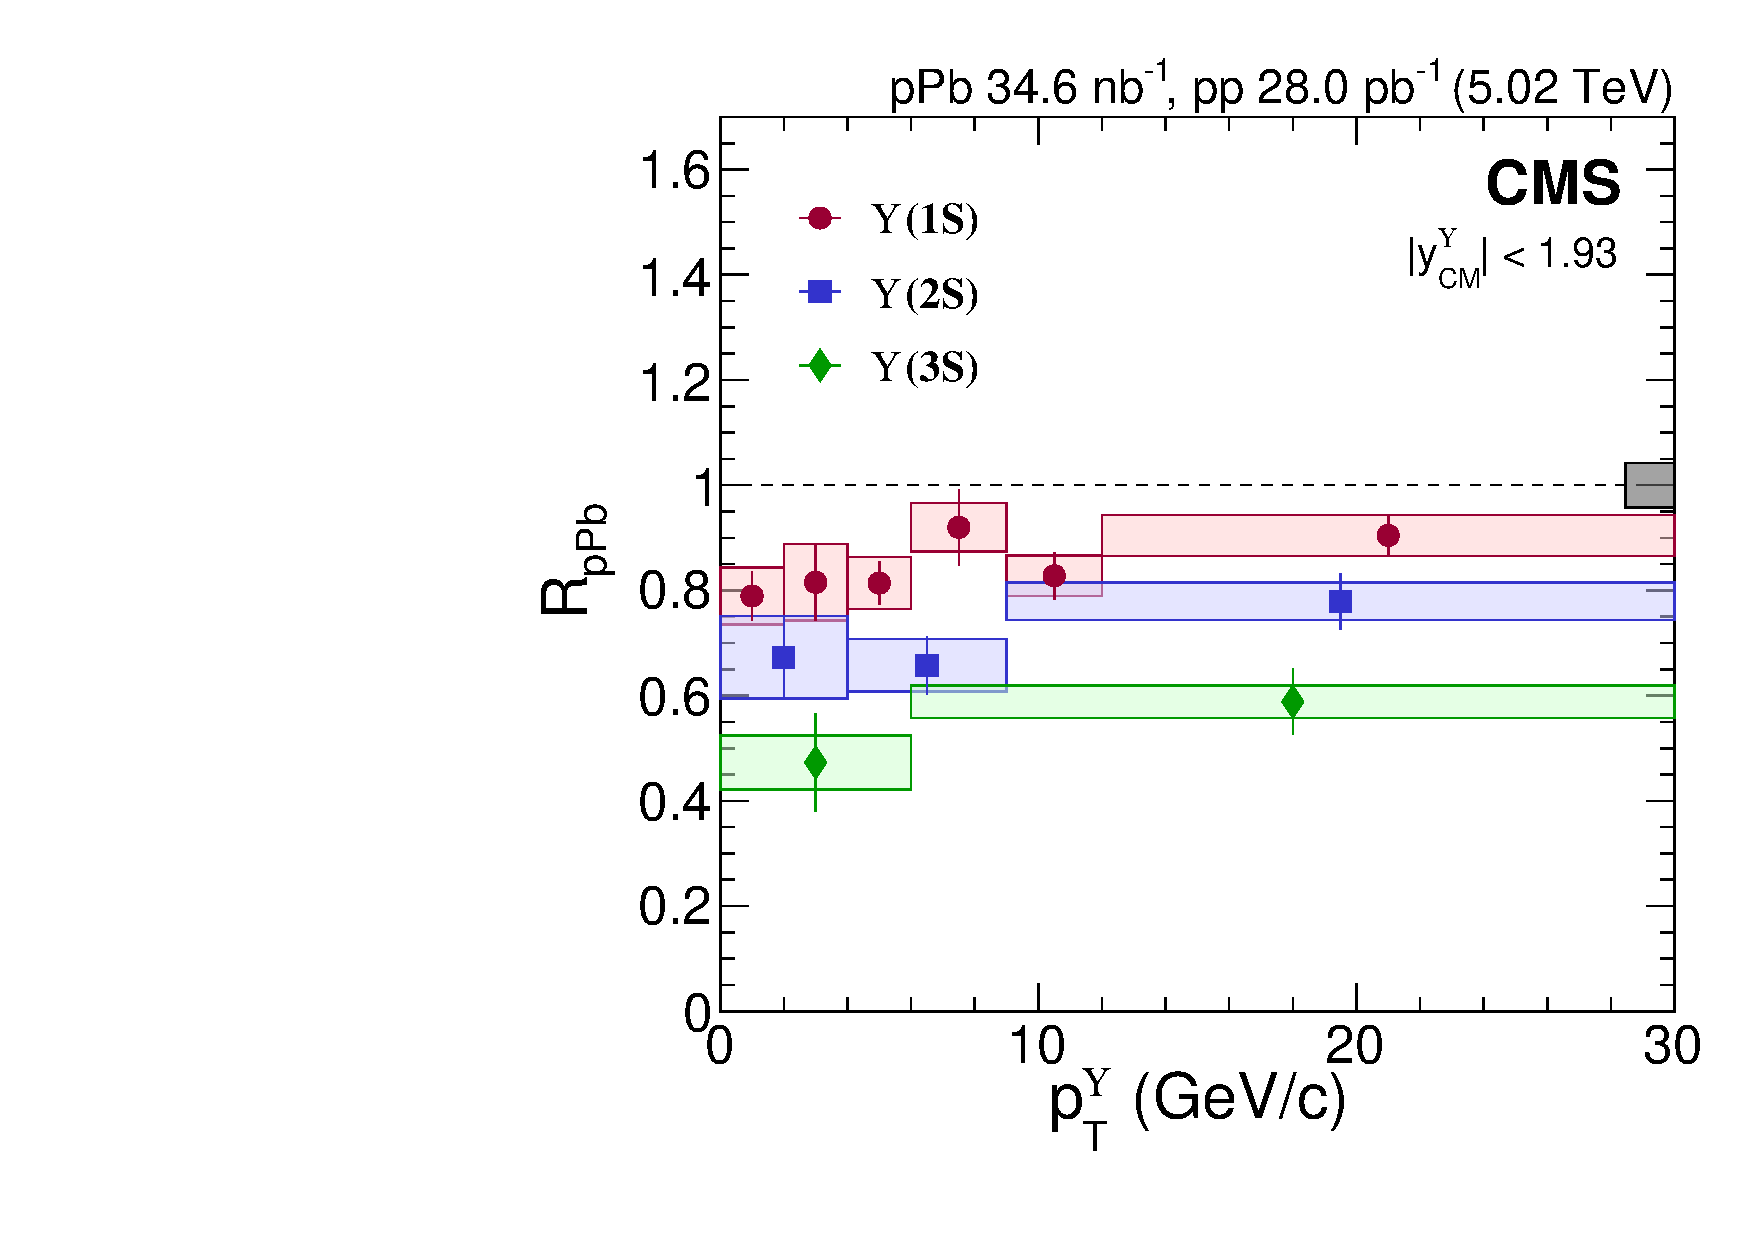
\includegraphics[width=0.49\textwidth]{Figures/ExpOverview/CMS-HIN-18-005_Figure_003-a.pdf}
    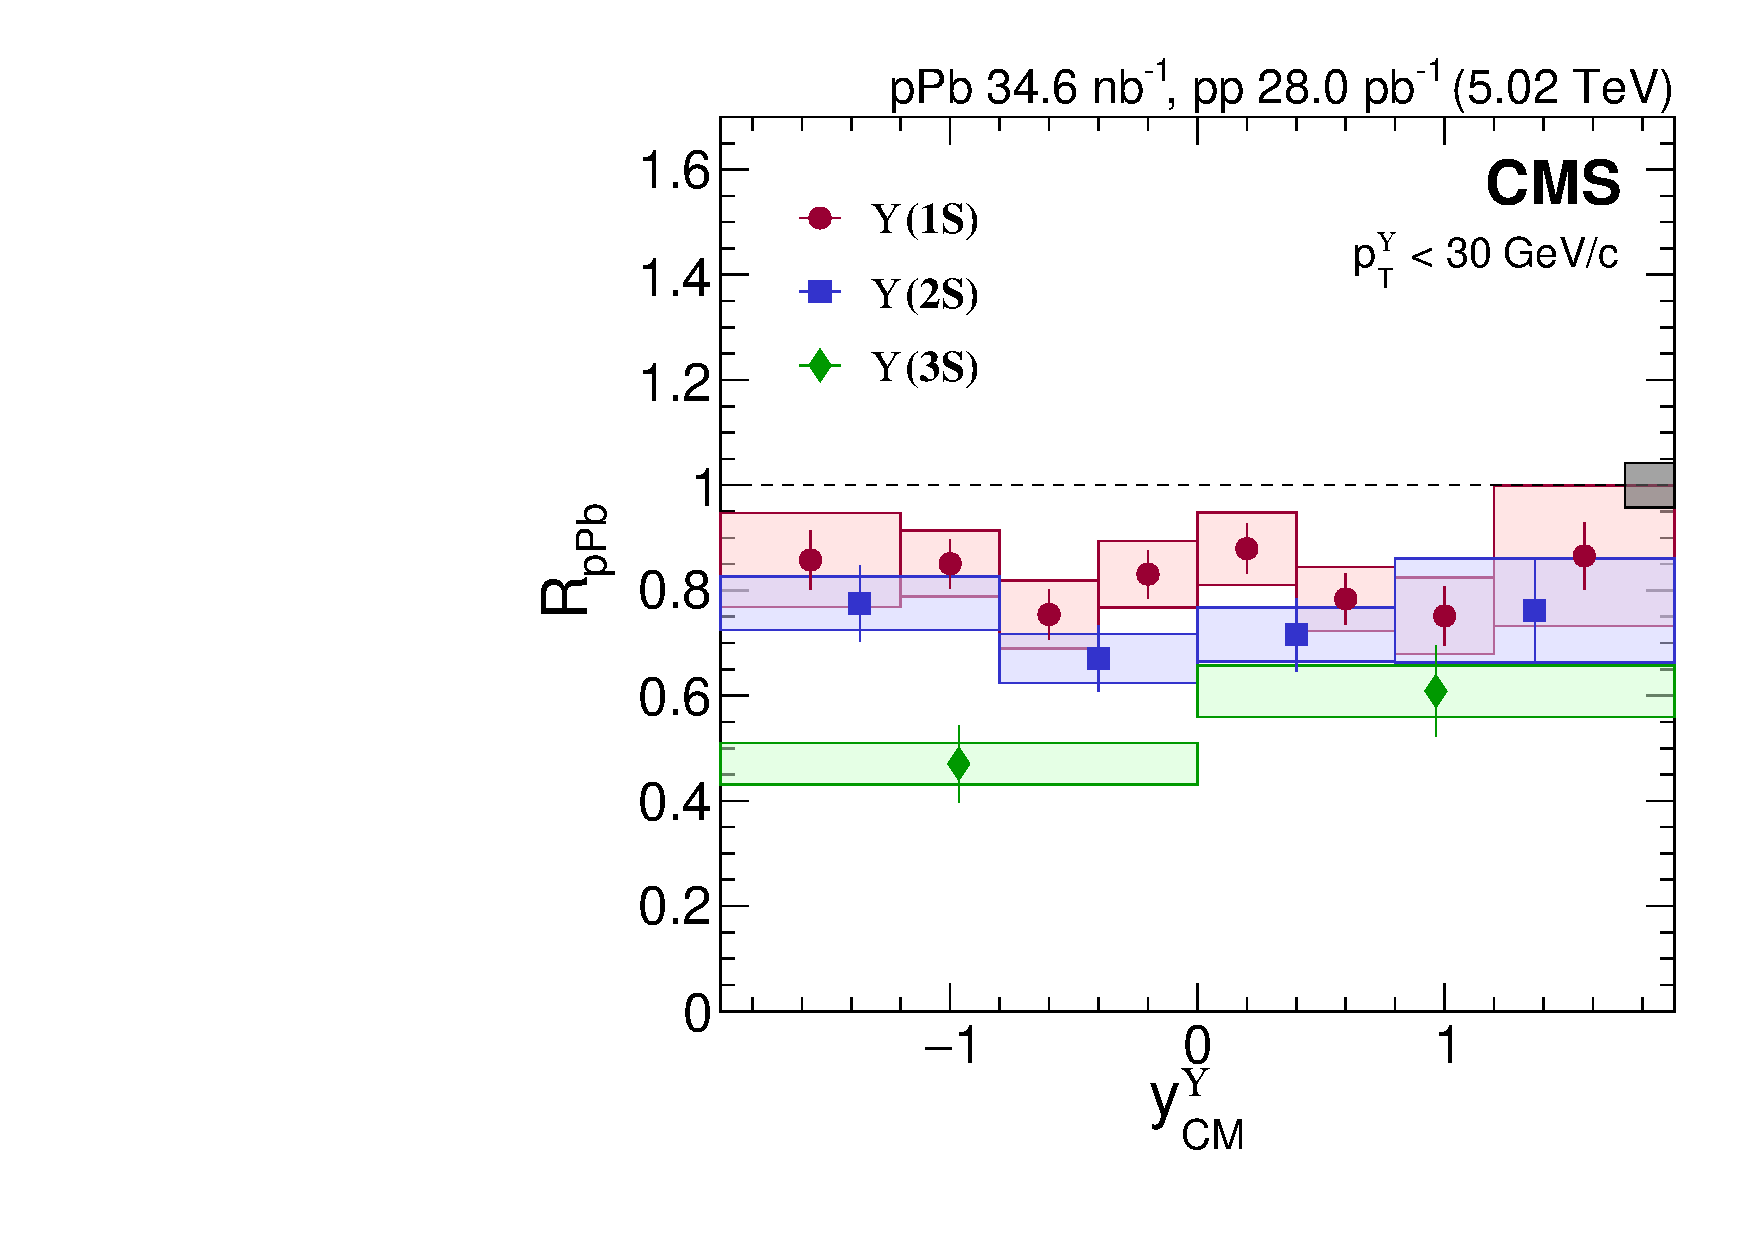
\includegraphics[width=0.49\textwidth]{Figures/ExpOverview/CMS-HIN-18-005_Figure_003-b.pdf}
    \caption{(Color online) The $\Upsilon$(nS) nuclear modification factor, $R_{pA}$,
      (a) as a function of transverse momentum $p_{T}$
    and (b) as a function rapidity in pPb colisions at 5.02 TeV measured by CMS~\cite{CMS:2022wfi}
  }
  \label{fig:LHCpPb5}
\end{figure}



\begin{figure}
  \begin{center}
  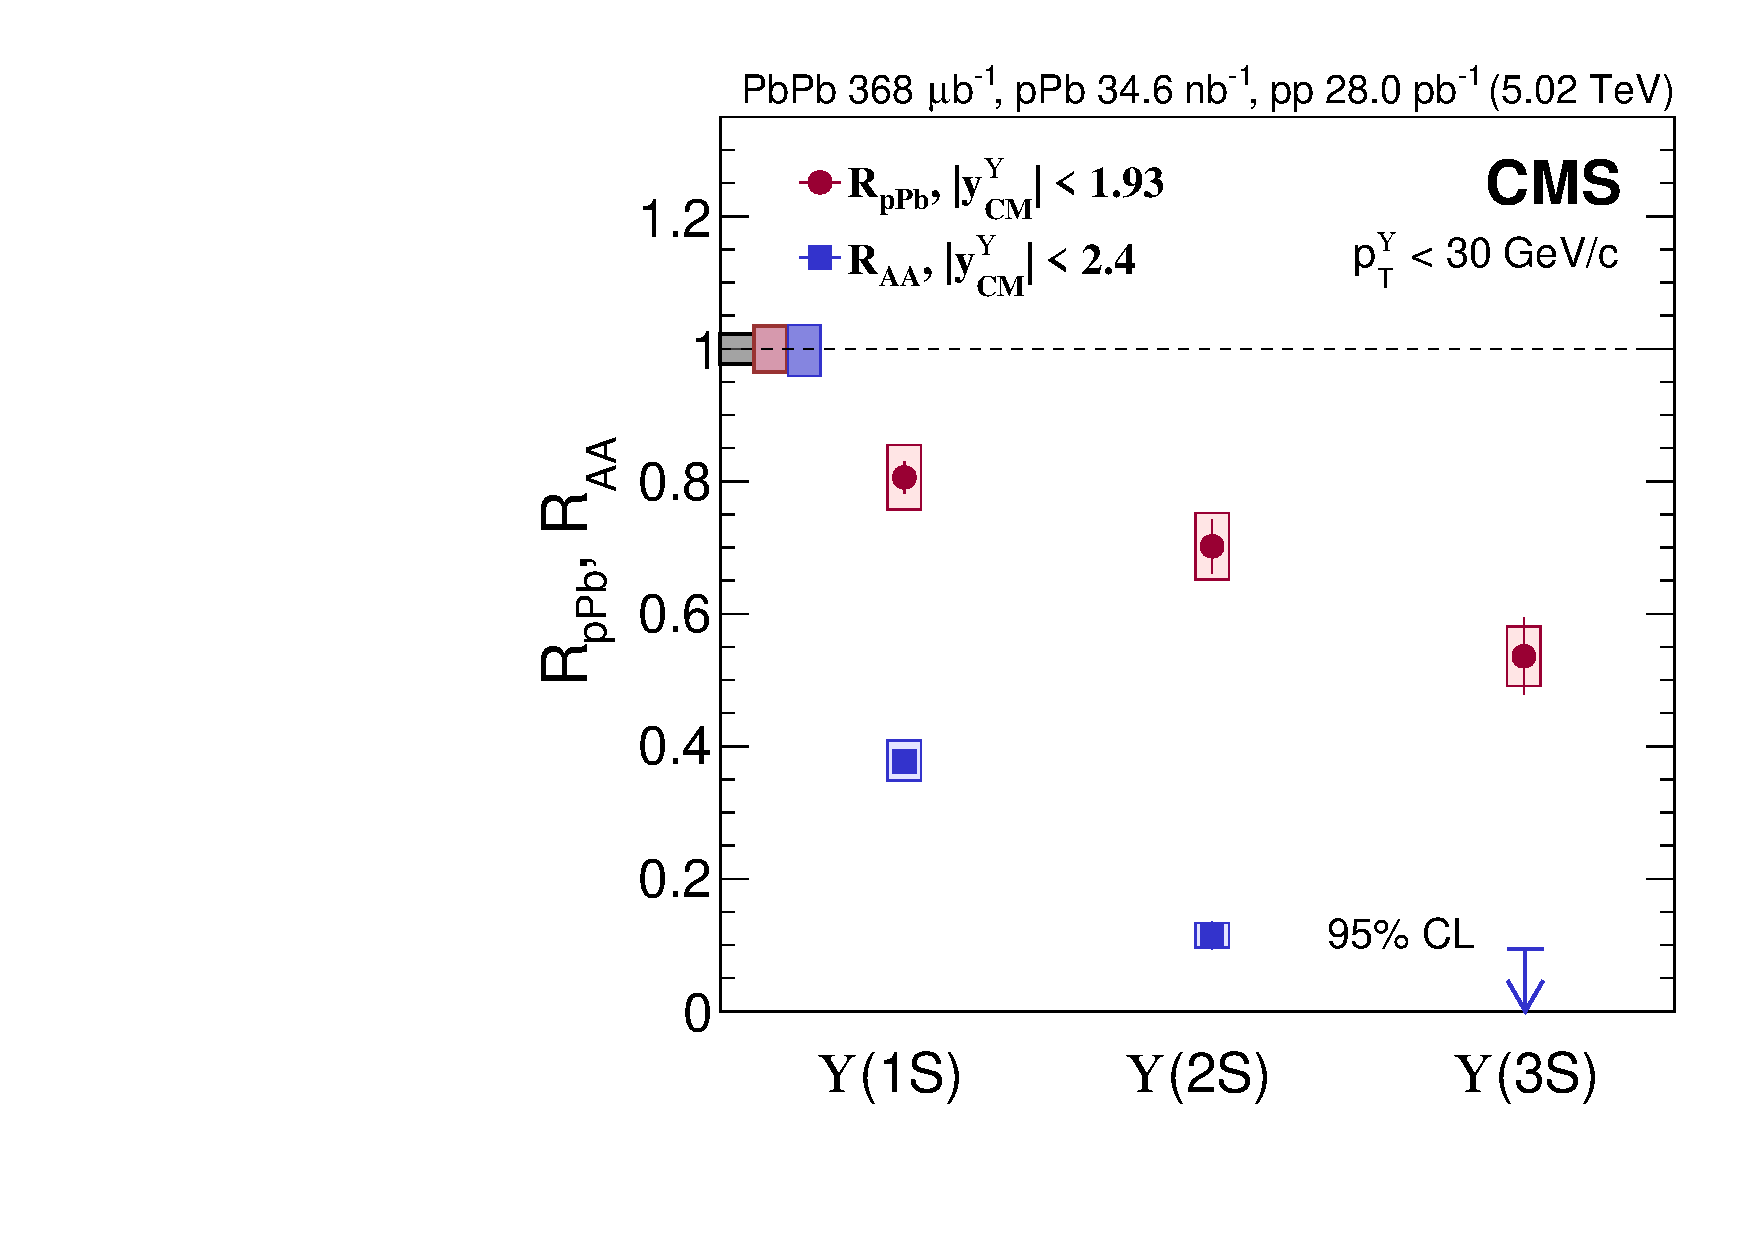
\includegraphics[width=0.60\textwidth]{Figures/ExpOverview/CMS-HIN-18-005_Figure_008.pdf}
  \caption{(Color online) The $\Upsilon$(nS) nuclear modification factors,
    $R_{pA}$~\cite{CMS:2022wfi} and $R_{AA}$~\cite{CMS:2018zza}
    at 5.02 TeV measured by CMS.
  }
  \end{center}
 \label{fig:LHCpBPbPb}
\end{figure}



  
